\documentclass[a4paper,11pt]{report}

\usepackage{times}
\usepackage[numbers]{natbib}
\usepackage[pdftex]{graphicx}
\usepackage{epstopdf}
\usepackage{algorithm}
\usepackage{algorithmic}
\usepackage{amsmath}
\usepackage[section,subsection,subsubsection]{extraplaceins} %http://lexfridman.com/blogs/research/2011/03/06/prevent-figures-from-floating-outside-sections-in-latex/

\title{Using Competence Models in Active Learning}
\author{Charles McCarthy\\
  106380221\\
  \texttt{cmmc1@student.cs.ucc.ie}
  \\Supervisor: Dr. Derek Bridge}
\date{March 2012}

\usepackage{hyperref} % Taken from Barry Hurley
\hypersetup{colorlinks,%
	    citecolor=black,%
	    filecolor=black,%
	    linkcolor=black,%
	    urlcolor=black}

\begin{document}

\maketitle

\begin{abstract}
An overview of the fundamental concepts in Active Learning, with particular focus on the use of Competence Models. Experimental analysis of basic Selection Strategy approaches, along with experiment on new Competence Model based approaches.
\end{abstract}

\chapter*{Declaration of Originality}
\vspace*{\fill}
In signing this declaration, you are confirming, in writing, that the submitted work is your own original work, unless clearly indicated otherwise, in which case, it has been fully and properly acknowledged.

I hereby declare that:
\begin{itemize}
	\item this is all my own work, unless clearly indicated otherwise, with full and proper accreditation;
	\item with respect to my own work: none of it has been submitted at any educational institution contributing in any way towards an educational award;
	\item with respect to another's work: all text, diagrams, code, or ideas, whether verbatim, paraphrased or otherwise modified or adapted, have been duly attributed to the source in a scholarly manner, whether from books, papers, lecture notes or any other student's work, whether published or unpublished, electronically or in print. 
\end{itemize}

\vspace{\stretch{1.0}}
{
\renewcommand{\arraystretch}{4.5}
\begin{center}
 	\begin{tabular}{l @{:} p{0.4in} l}
		Name & & Charles McCarthy \\
		Signature & & \makebox[2.5in]{\hrulefill} \\
		Date & & March 2012 \\
	\end{tabular}
\end{center}
}
\vspace{\fill}

\chapter*{Acknowledgements}
While much of the work carried out was based on external literature, a great deal of advice and direction was gained from the weekly meetings with my project supervisor, Dr. Derek Bridge.

The impact of casual conversations with classmates P\'{a}draig \'{O}'D\'{u}inn, Barry Hurley and Kevin Leo should also be acknowledged. P\'{a}draig, in his research, encountered similar issues to myself on occasion, and would often share his insights into how he got around them. Barry was useful in offering Latex help, and was sometimes consulted while I was learning it. Kevin had a great deal of python and general *nix experience, and offered advice and assistance whenever particularly frustrating issues were encountered (which would usually be prompted by me ranting about them during our lunchtime card games).

\tableofcontents

\chapter{Introduction}
\section{Active Learning Overview}
The key concept of Active Learning is that a machine learning program has a say in its own learning process, by being capable of choosing the data from which it learns. 

This concept fits particularly well in the domain of Case Based Reasoning Systems. In Case Based Reasoning Systems, the system has a pool of cases for which it knows the label. When an unlabelled case is presented to the system, the system uses this pool to try to guess the label of the unlabelled case.

The facet of Active Learning we will subsequently consider is known as Pool Based Sampling in other literature \cite{Settles2010}, and is based on the idea that there is a large quantity of unlabelled cases available, but getting labels (or more likely, consulting a Human Expert) is an expensive process, for which it is undesirable to apply to the entire unlabelled set. The aim for the system is to choose a subset of these unlabelled cases for which to request a label. These are then used as the system's pool of labelled cases which it will consult in future.

The system would like to maximize its classification accuracy for future instances, but have to resort to asking the Oracle external to the system for a minimal number of labels.

For an in-depth review of Active Learning, and some of the recent Active Learning literature, consult \citep{Settles2010}.

\section{Importance of Active Learning}
There are many real-world domains in which a large quantity of unlabelled data is available, but the process of manually labelling all of that data is not feasible. 

A Human Expert is often needed to label instances of the data. This human factor limits the quantity of data which can be labelled. The financial cost can be significant, and the availability of such an expert can also be a limiting factor.

Often the labelling process is in itself exceedingly slow compared to either the amount of unlabelled data available, or the rate at which new data is being generated. 

Machine Learning seems a clear answer for these type of scenarios, but for Machine Learning, one still needs training instances to initially train the system.

\subsection{Examples of Active Learning Domains}
\subsubsection{Recommendation Engines}
In recommendation engines, the user can be thought of as the Oracle. It is from user feedback (either implicit or explicit) that the recommendation engine can know if an item was relevant to the user or not. It is likely that there is a vast library from which a recommendation can come, but the quantity of user feedback may be limited.

What is sometimes done in these systems is that the engine includes some results it is relatively certain will be relevant to the user, but others of which it is uncertain, but would like to gain feedback on from the user. Only comparatively few of these instances can be given to the user for feedback, as doing otherwise would negatively impact the user's experience.

Choosing which uncertain instances to present to the user to maximize the system's competence-gain is therefore an important problem for the system.

\subsubsection{Medical Data}
Medical data is another area in which Active Learning is of particular interest and relevance.

Vast quantities of patient data exists, but each patient data instance is unlikely to have results of tests for every possible disease / condition. It is obviously preferable though to detect any illness or condition a person has as soon as possible, so that appropriate measures are taken. It is not feasible however to test each individual for every possible illness.

When building a system to predict illnesses, one would want to minimize the number of physical tests to be carried out on patients for the purpose of training the system. It is in this way that Active Learning can have a useful role to play.

\subsubsection{Computer Vision}
Computer Vision is another area in which large quantities of data are available, and easy to generate, but manual labelling is incredibly tedious.

\subsubsection{Text Classification}
Increasingly with the proliferation of the internet, and in particular social media, text classification has many practical applications. The traditional example is that of email spam analysis, but more and more, sentiment analysis is becoming an active area of interest.

Vast quantities of textual data are often available for the target domain, though initial labelling requires human involvement. Active Learning thus has a potentially very useful role in the process, helping in maximising the system gain with the minimum of data.

\subsubsection{Voice Analysis}

Speech recognition is one area that can bring immense benefit to users, but for which manual labelling requires expert skills, and is painstakingly slow even with a trained expert's involvement. For such systems, it is highly desirable to reduce the quantity of data that must be manually labelled to bring the system to an acceptable rate.

\section{Fundamental Concepts}
\subsection{Pool Based Active Learning}
In particular, we concern ourselves with \emph{Pool Based Active Learning}, and it is in this context that further concepts should be taken.

In Pool Based Active Learning, a Pool of Unlabelled Cases are available, from which the System may choose Instances to request a Label for. The System uses these Labelled Instances to train a Classifier.

\begin{figure}[h!]
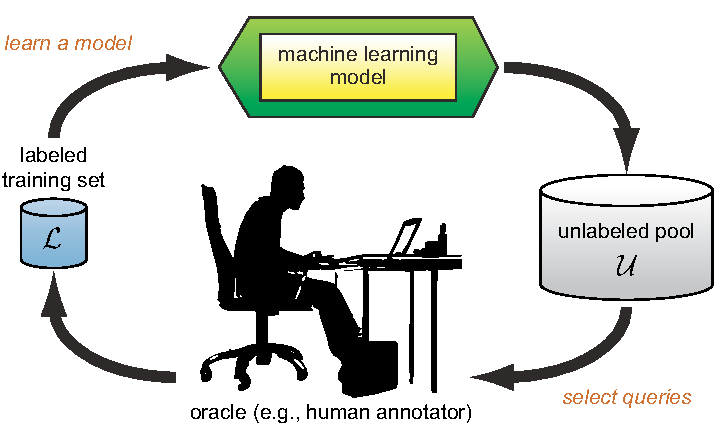
\includegraphics[width=10cm]{./Others/Settles2010PoolBasedImage}
\caption{Pool Based Active Learning Cycle Diagram found in \citep{Settles2010}}
\end{figure}

\subsection{Case Base}
The Case Base is the labelled pool of data which the overall system consults when a new unlabelled instance is presented for classification.

\subsection{Case-Based Classification using kNN}

A k Nearest Neighbours approach fits the Case Base concept quite well. When a new unseen Instance is presented to the Classifier, the Classifier can simply walk through the Case Base to find Cases which are similar to the presented Case. It can then use these Labelled Cases in some sort of Voting fashion to Classify the presented Case.

When new data is added to the Case Base, there is no real cost in re-training the Classifier, since re-training simply involves adding the new data to the set in which the kNN walks through (which can simply be the Case Base itself).

\subsection{Oracle}
The Oracle is the entity which the system may consult if it wishes to determine the true label for an instance.

Often, the Oracle is a Human Expert familiar with the domain who must manually classify the instance. Though the Oracle may also just be another system, but for which there is some expense in using to determine a class. \footnote{Here, we use the word `expense' in its broadest possible meaning. It may be financially expensive, computationally expensive, or simply take an exceedingly long amount of time to run. In any event, `expense' refers to some undesirable operation for which we want to minimise the number of calls.}

\subsection{Selection Strategy}
While the term Selection Strategy can have slightly different meanings given the type of Active Learning being considered, we will subsequently use the phrase to mean the algorithmic approach taken to determine which unlabelled instances to query with the Oracle for the true label.

\subsection{Stopping Condition}
The Stopping Condition of the system is the point at which the system must stop consulting the Oracle.

\subsubsection{Examples of stopping conditions}
\paragraph{Oracle Budget} 
The Oracle is willing to classify only a fixed number of instances.

\paragraph{Desired Classification Accuracy} 
The system stops asking the Oracle for a Label after it is capable of achieving a certain classification accuracy on its test set.

\section{Variations / Related Areas}
Many variations on the concept of Active Learning exist. The following is intended to give just a small subset of examples, as opposed to an exhaustive listing. Further information can be gleaned from \citep{Settles2010}.

\subsection{Case Base Maintenance}
Case Base Maintenance is concerned with the task of how to maintain a case base. 

Over time, as new instances are added, the case base size increases. This can have an adverse effect on system performance, thus it can be desirable to have the case base be as minimal as possible, while maintaining classification accuracy.

Another consideration is that some cases may be adversely affecting the system's classification accuracy. It may be that these instances were initially misclassified by the Oracle, the underlying data was noisy, or it could be that the nature of the domain has changed and that similar instances now actually have a different label. The detection of these cases is therefore an important part to long-running Case Based Reasoning Systems.

Overall, Case Base Maintenance can be summarised as the process of maintaining a case base to a desirable level over time. This contrasts to what we will concern ourselves with - how to build a Case Base.

\subsection{Seeding in Active Learning}
Many Selection Strategies have the assumption built in that there are already some cases in the case base from which they may base their judgements. Thus the issue how to initially seed the Case Base crops up.

In our evaluations and experimentation, we don't attempt to initially seed the Case Base - instead starting with an empty Case Base. The reasoning for this is twofold: 
\begin{enumerate}
	\item The datasets we use are relatively simplistic, which even with random sampling, converge to a relatively high accuracy even after a small number of samples are added. This would make it very difficult to reasonably compare different selection strategies. 
	\item Adding Seeding would also add another factor for testing, as opposed to primarily testing the variance between different Selection Strategies.
\end{enumerate}

\subsubsection{Examples of Seeding Strategies}
\begin{itemize}
	\item Random Seeding
	\item K Means
	\item K Medoids
\end{itemize}

\subsection{Stream Based Learning}
In this methodology, the system does not just select at the outset from an unlabelled pool the instances to request classification by the Oracle. Instead, It is presented with a stream of instances, and for each instance, it may either itself guess the classification (if it is relatively sure it is correct), or it may defer the decision to the Oracle.

This notion can sometimes be more useful - but it is unlikely in practice that the system would query at any arbitrary time for a Label from the Oracle, since with the usual case of requiring human involvement, the Oracle may not be available at all times.

What is more likely is that the system would keep note of instances it is very unsure of, guess the classification anyway if an immediate response is required, and at the next opportunity, query the oracle in batch regarding the true classification.

\subsection{Query Synthesis}
Although it can cause hassle for a human annotator, another variation is known as Query Synthesis, in which the program actually constructs its own unlabelled data instances to present to the Oracle (as opposed to the data being actual previously observed).

The program is thus able to actively explore the domain space, as opposed to just waiting for data to try to infer this information.

While unsuitable for many problem areas (in particular text), one could easily see how this model could be useful in the context of scientific experiments. The program may wish to make \emph{guesses} as to what would be useful data to get \emph{classified}, so that it may further refine it's knowledge of the domain.

\citep{Settles2010} points to a good example involving a ``robotic scientist'' as described in \citep{King2009}.

Query Synthesis is not really necessary in tradition Pool Based Sampling areas - since a large pool of truly observed (and therefore valid) unlabelled examples are present that should be representative of the type and distribution of problems which will be later presented to the system.

\subsection{Batch Learning}
In practice, it is unlikely that instances would be presented to the Oracle one-at-a-time. What is more likely is that batches of instances are presented to the Oracle.

In our investigation, we do not perform batch learning - instead presenting instances one at a time to the Oracle (equivalent to a batch size of 1).

\subsection{Noisy Oracle}
A \emph{Noisy Oracle} relates to the Oracle being wrong in its classification some of the time.

In our investigation, we do not deal with this variation at all, assuming a Perfect Oracle.

\subsection{Classification Cost Variation}
In many real-world applications, the cost associated with classifying an instance can vary from instance to instance. Some instances can involve much more time to determine a Label for than others. In text classification, articles vary in length and complexity. Similarly in video and audio.

This paper does not deal with instance classification cost variation, instead assuming a fixed cost.

\section{Report outline}
\begin{itemize}
	\item Chapter \ref{cha:litreview} will outline various basic Selection Strategies as found in existing Active Learning Literature, as well as looking at some more complicated strategies.
	\item Chapter \ref{cha:platarch} will give an overview of the Platform Architecture developed during the course of this project for running and analysing Selection Strategy experiments.
	\item Chapter \ref{cha:CompetenceModels} will introduce the notion of Competence Models, outlining a particular Model developed by a researcher from DIT. It will then proceed to present our attempts at expanding the models, and using them in an Active Learning context.
	\item Chapter \ref{cha:expanalysis} will present the results of the Experimental Analysis carried out on the basic Selection Strategies, and our Competence based Strategies.
	\item Chapter \ref{cha:conclusions} finishes with the conclusions to the Project, and potential areas of future work that could in theory follow.
\end{itemize}

\chapter{Literature Review\label{cha:litreview}}

\section{Common Concepts}
Certain concepts very frequently occur in the Active Learning Literature, so these will be outlined first.

\subsection{Similarity/Distance}
The notion of Similarity or Distance between pairs of data instances is often core in many Selection Strategies. As one would expect - the Similarity between two data instances is a numerical figure which represents how similar the instances are to one another.

Distance is simply the inverse of Similarity, representing numerically how far two data instances are away from each other.

\subsection{(Nearest) Neighbours / Neighbourhood}
It is common to define a group of cases relative to an individual case that in some fashion relate more strongly to the case than other cases in the Case Base - cases that \emph{neighbour} that case by means of the relation.

Nearest Neighbours follow fluidly from the use of k-Nearest Neighbour style classification approaches that often go along with Case Based Reasoning Systems, and are sometimes used for additional purposes.

Neighbourhoods based on other characteristics such as Shared Coverage can also be defined.

\subsection{Density}
The notion of Density is extremely common. It simply represents how dense a region is within a group.

Density is usually measured across the entire data set (i.e. both the unlabelled and labelled pool), as it is of less use to know of dense regions within the labelled dataset when trying to choose instances from the unlabelled data to request a label for\footnote{This at least is the case when building the case base. For case-base maintenance tasks, dense regions within the case-base might indicate redundancy.}. 

The reasoning is that the entire data-set is hopefully representative of real-world instances, of which new instances will appear with similar ranges and distributions. If one selects from a dense region of the unlabelled dataset, it would be hoped that it would cover a large range of input problems.

Even with the commonality of the Density notion, there is variance in the literature around how density is actually measured. Two examples of relatively straightforward measures:
\begin{enumerate}
	\item \textbf{Global Density}: Represented as the average distance from an instance to every  instance in the data set\cite{Xu2007}.
	\item \textbf{Local kNN Based Density}: Represented as the average distance to its k nearest neighbours within the data set.\cite{Zhu2008}.
\end{enumerate}

Density is also sometimes measured for groups as opposed to on a case-by-case basis\cite{Smyth1998}, and often involves the sum of the pair-wise Similarities for the cases in the group.

\subsection{Diversity}

Diversity (usually also mentioned with Density) is another common measure used. It simply represents how different a case is compared to other cases in a group.

In contrast to density, diversity is usually not measured across the entire data-set, but instead just across the actual Case Base\footnote{Again, this might not be the case when one is dealing with Case Base Maintenance.}. The reasoning for this is that it would be beneficial to select new instances that are diverse from what is already present in the Case Base, in hopes that a larger range of the domain may be solved as a result. 

\subsection{Solves / Classifies / Contributes}
When it comes to analysing an individual Case, often the notion of the other Cases that the individual Case can somehow Classify comes into question. In the context of kNN Classification though, an individual Case will not be able to Classify another case on its own, instead somehow only possibly contributing to another Case's Classification. This leaves room for different definitions of what one means when they consider a Case capable of Solving another Case. 

\citep{BridgeUpcoming} highlights the interesting point that there are subtle but definitely significant differences to what different researchers mean when they use the term Solves. Often, they seem to be glossed over quickly in literature due to their apparent obviousness, but are often core to the algorithms presented.

\subsection{Clustering}
Somewhat related to Density, Clustering is sometimes performed on the data set. Usage of clustering varies massively, but one relatively common use is to use Cluster-centres from dense regions as initial seeds for the case base.

\section{Basic Selection Strategies}
\subsection{Random Sampling}
\emph{Random Sampling} is probably the most basic Selection Strategy. It simply select Instances at random from the Unlabelled Set. Even with its simplicity, it has the benefit of resulting in a moderately representative sampling of the domain\footnote{This is assuming that the Unlabelled Instances are a representative sampling of the real world domain - which we usually assume that they are.}.

It is often used as one of a group of baseline strategies on which other strategies are compared.

\subsection{Uncertainty Sampling}
\emph{Uncertainty Sampling}\cite{Lewis1994} selects Instances that a Classifier trained on the Case Base is most uncertain about (or said another way - is least certain about). Assuming the Classifier can generate a probability for each Label when provided with a new Instance, the maximum of these for an Instance can be said to be the \emph{certainty} with which the Classifier can classify that Instance.

The benefit of Uncertainty Sampling is that it doesn't select redundant instances, since whatever it selects is the one that it is least capable of Classifying with its current Case Base. The downside is that it is very prone to querying outliers, since it does not consider information such as the density of the region from which the Instance comes.

Uncertainty Sampling, like Random Sampling, is very commonly used as a baseline when evaluating new Algorithms.

\subsection{Uncertainty with Density}
As discussed in the previous section, Uncertainty Sampling has the serious downfall of being prone to querying outliers, since it does not consider the region surrounding the Instances it selects.

A very straightforward attempt at solving this issue is by incorporating Density information also, giving an additional weighting to the Uncertainty measures based on how Dense a region the Instance in question comes from. Uncertain instances from dense regions thus become more favourable than Uncertain instances from very sparse regions (outliers).

One example of combining Uncertainty with Density can be found in \citep{Zhu2008}, though it uses an Uncertainty measure based on Entropy as opposed to pure Uncertainty alone.

\subsection{Margin Sampling}

\emph{Margin Sampling} tries to account for a shortcoming in pure Uncertainty Sampling for Multi-label Classification in that it only considers information about the most probable label, essentially throwing away the information about the other labels.

Margin Sampling looks at the difference between the probability of the most probable label, and the second most probably label. The intuition is that if there is a large difference between the two, the Classifier must be relatively certain. Whereas if there's very little difference, then with relatively little change, the Classifier might could have picked a different Label, and so it really mustn't have been very certain about it.

Margin Sampling really only makes sense in Classification where there are more than two possible label values. In Binary classification, Margin Sampling gives an identical strategy to Uncertainty Sampling.

\subsection{Diversity Only}
In a \emph{Diversity Only} Sampling, the System selects Instances that are as far away as possible from everything else in the Case Base. This can result in an understandably Diverse Case Base, but is very prone to querying outliers like Uncertainty Sampling.

This motivates many authors to try and incorporate Density information with Diversity. One such attempt is described below.

\section{Rong Hu's Work on EGAL: Exploration Guided Active Learning}
\subsection{Introduction}
Many Selection Strategies have firm dependencies on a type of Classifier confidence score (what Hu terms Exploitation Strategies), while also incorporating measures such as Density and Diversity (what Hu terms Exploration Strategies).

Hu, in her work on EGAL, experiments with developing an Exploration only strategy by using only a combined measures of Density and Diversity\footnote{Rong Hu recently completed her PHD Thesis on ``Active Learning for Text Classification'' in D.I.T. with Dr. Sarah Jane Delaney as one of her supervisors \cite{Hu2011}. In her thesis, she covers a broad range of topics, but of particular interest to us is her work on ``EGAL'', and also on using Aggregate Confidence Measures.}.

While some of the formula specifics feel slightly odd, the overall attempt on using an Exploration only strategy is pretty interesting. 

%TODO Density + Diversity - needs a bit more explanation.

\subsection{Density}
\[
density(x_{i})=\underset{x_{r}\in N_{i}}{\sum}sim(x_{i},x_{r})
\]

\[
N_{i}=\left\{ x_{r}\in D\mid sim(x_{i},x_{r})\geq\alpha\right\} 
\]

$\alpha=\mu-0.5\times\delta$ where $\mu$ is the mean, and $\delta$ is the standard deviation of the similarities. This value for $\alpha$ is somewhat arbitrary, in that it just seemed to work well in Hu's experiments.

Of particular note is that the density measure is calculated across the entire dataset (i.e. unlabelled + labelled). This being in contrast to the upcoming Diversity measure - which is measured just on the labelled instances.

\subsection{Diversity}

\[
diversity(x_{i})=\frac{1.0}{max_{x_{r}\in L}sim(x_{i},x_{r})}
\]

It's inverted because distance is inverse of similarity. So diversity is really the distance to the nearest neighbour in the Labelled set.

\subsection{Combining Density and Diversity}

\subsubsection{Candidate Set}
\[
CS=\left\{ \exists x_{i}\in U\mid diversity(x_{i})\geq\frac{1}{\beta}\right\} 
\]

This is presented in a slightly expanded (but equivalent) form in Hu's paper dedicated to EGAL\cite{Hu2010}. Really, $\beta$ represents the maximum similarity allowed to its nearest neighbour. This formula forms the set of cases which do not have any other cases within a distance of $\frac{1}{\beta}$.

It will be from the Candidate set that instances will be selected - but more on that below.

\subsubsection{Generating the Max Similarity Sets}

Firstly, for each item in the Unlabelled set, the similarity to the \emph{closest} element in the labelled set is calculated and stored. \footnote{Diversity is the distance to the closest element. The inverse of distance gives similarity. Thus the inverse of diversity is the Similarity of an element to its closest element.}

\[
S=\left\{ s_{i}=\frac{1}{diversity(x_{i})}\mid x_{i}\in U\right\} 
\]

\subsubsection{Determining $\beta$}
A proportion $w$ is chosen from experimentation. It will represent the proportion of the top-most diverse elements to include in the Candidate Set.

\[
S_{1}=\left\{ s_{i}\in S\mid s_{i}\leq s_{w}\right\} 
\]

\[
S_{2}=\left\{ s_{j}\in S\mid s_{j}>s_{w}\right\} 
\]

\[
\left|S_{1}\right|=\left\lfloor \left(w\times\left|S\right|\right)\right\rfloor +1,\hphantom{}0\leq w\leq 1
\]

It does this by choosing a similarity value $s_{w}$ that would give that proportion. $\beta$ is then set to that $s_{w}$ value.

\subsubsection{Algorithm Outline}
\begin{enumerate}
	\item Initially $\beta$ is simply set to $\alpha$, but is updated according to the formula above each time to candidate set becomes empty.
	\item The candidate is sorted from highest density to lowest density, and items are taken in order until the stopping condition is reached.
\end{enumerate}

\subsubsection{Factor Summaries}
\begin{itemize}
	\item $\beta$ relates to the minimum distance  that labelled examples should be from an unlabelled example for it to be thought of as \emph{diverse}, and thus should be included in the \emph{Candidate Set}.
	
	This is represented in terms of similarity - the maximum similarity.

	\item $\alpha$ relates to the distance (really similarity) within which to define the neighbourhood of an instance for the purpose of calculating the density (total pairwise similarity) of the instance. 
	
	This is represented in terms of similarity - the minimum similarity value instances should have to be within the neighbourhood.
	
\end{itemize}

\subsubsection{$w$ as a Density/Diversity Balancing factor}
Hu explains that $w$ is a balancing factor between Density and Diversity\cite{Hu2010}. 

\begin{itemize}
	\item When $w=0$, a pure diversity-sampling approach occurs. 
	\item When $w=1$, a pure density-sampling approach occurs. 
	\item When $w$ is set to values between $0$ and $1$, a mixture of density and diversity sampling occurs.
\end{itemize}

\subsection{Experimental Results}
In \citet{Hu2011}, Hu finds that w=$0.25$ gives the best results for the data sets she used. She also finds that 

Hu also finds that the EGAL strategy with $w=0.25$ compares favourably with Random Sampling, and also beats Diversity-only and Density-only sampling.

For comparison with other Active Learning strategies, Hu finds that EGAL performs generally better than the other strategies at the initial stages of the Active Learning process.

\subsection{Comments}
Even though $w=0$ gives a diversity-only approach, and $w=1$ gives a density-only approach, it is unclear the exact effect of having values in between the $0$ to $1$ range.

\section{Rong Hu's Work on Using Aggregate Confidence Measures}
\subsection{Introduction}

\subsection{Model \& Measures}

In \citet{Delany2005} - Delany proposes five confidence measures. Hu chooses the three of these which she determines experimentally to have the least correlation.

For the three, the following metrics are needed:
\begin{itemize} 
	\item $N_{i}(t)$ denotes the ith nearest neighbour of example t.
	\item $NLN_{i}(t)$ denotes the ith nearest like neighbour to example t.
	\item $NUN_{i}(t)$ denotes the ith nearest unlike neighbour to example t.
\end{itemize}
%TODO Needs more explanation
\subsubsection{Average NUN Index} \footnote{The measure is based just on indexes. It seems slightly strange to just use indexes, not considering the density, etc. of the neighbours. The validity / appropriateness of this approach will not be considered further though - since this particular paper - and the piece of interest to us - is that of aggregating confidence measures.}

\[
AvgNUNIndex(t,k)=\frac{\sum_{i=1}^{k}IndexOfNUN_{i}(t)}{k}
\]

where:
\begin{itemize}
	\item $IndexOfNUN_{i}(t)$ is the index of the ith nearest unlike neighbour of target example t, the index being the ordinal ranking of the example in the list of NNs
\end{itemize}

\subsubsection{Similarity Ratio}
\[
SimRatio(t,k)=\frac{\sum_{i=1}^{k}Sim(t,NLN_{i}(t))+\epsilon}{\sum_{i=1}^{k}Sim(t,NUN_{i}(t))+\epsilon}
\]

where:
\begin{itemize}
	\item $Sim(a, b)$ is the similarity between examples $a$ and $b$ 
	\item $\epsilon$ is a smoothing value to allow for situations where an example may have no NLNs or NUNs ($\epsilon$ = 0.0001 is used in all of her evaluations). Top and bottom have this value to give a ratio of 1 when no NLNs or NUNs, since technically the ratio is 0:0 - a ratio of 1.
\end{itemize}

\subsubsection{Similarity Ratio Within K}
\[
SimRatioK(t,k)=\frac{\sum_{i=1}^{k}Sim(t,NN_{i}(t))\delta_{t,NN_{i}(t)}}{\epsilon+\sum_{i=1}^{k}Sim(t,NN_{i}(t))(1-\delta_{t,NN_{i}(t)})}
\]

where:
\begin{itemize}
	\item $Sim(a, b)$ is as above, 
	\item $\delta_{a, b}$ is Kronecker's delta where $\delta_{a, b}=1$ if the class of $a$ is the same as the class of $b$ and $0$ otherwise. 
	\item $\epsilon$ is a smoothing value to allow for situations where an example may have no NUNs ($\epsilon = 0.0001$ is used). \footnote{It's unclear the reason for the inconsistency between the use of $\epsilon$ on the bottom only here, but on top and bottom above.}
\end{itemize}


\subsection{Combining the confidence Measures}
\subsubsection{Initializing the Case Base}
Before the main algorithm which combines the confidence measures is initiated, the Case Base is initially seeded with a Deterministic variation on Furthest-First Initialization, as presented in \citet{Greene2007}

\subsubsection{Confidence Measure Threshold Initialization}
For \textbf{each} measure, the confidence threshold needs to identified for \textbf{each} class.

For each measure, predictions with confidence values higher than the predicted class's threshold are considered confident for that measure, while those with values below are considered non-confident for that measure.

Details surrounding how exactly these thresholds are set can be found in \citet{Delany2005}, but roughly, values are chosen on a per-dataset basis through experimentation. The experimentation, for binary classification\footnote{The false-positive analogy holds less for non-binary classification}, maximizes the correct classifications, while keeping the false-positives zero.

\subsubsection{Operation}
The algorithm essentially operates on (repeatedly) building 2 sets - the Confident Set, and the Non-Confident Set - from the Unlabelled data.

The Confident Set is composed of instances for which any their Confidence Measures exceeded the Measure's Confidence Threshold. The \emph{score} associated with each instance is the maximum of all the confidence measures for that instance.

The Non-Confident Set is composed of instances which do not appear in the Confident Set, but the \emph{score} associated with each instance is the minimum of all the confidence measures for that instance. 

This min-max combination was chosen as it performed the best in Hu's preliminary experiments when she considered multiple variations.\footnote{I really question this approach . . .}. Measures for each instance ``are normalised using statistical normalisation after performing a log transformation to correct those with skewed distributions''\cite{Hu2011}.

After the Confident and Non-Confident sets are built, selection begins. First elements in the Non-Confident Set are selected, and once it is expended, elements from the Confident Set are selected. Selection occurs from each of the sets in a lowest-score-first order. A batch size which is an input to the algorithm indicates how many should be selected in this \emph{batch}, before restarting the entire process, and beginning the selection of a new batch from the start again.

\begin{figure}[h!]
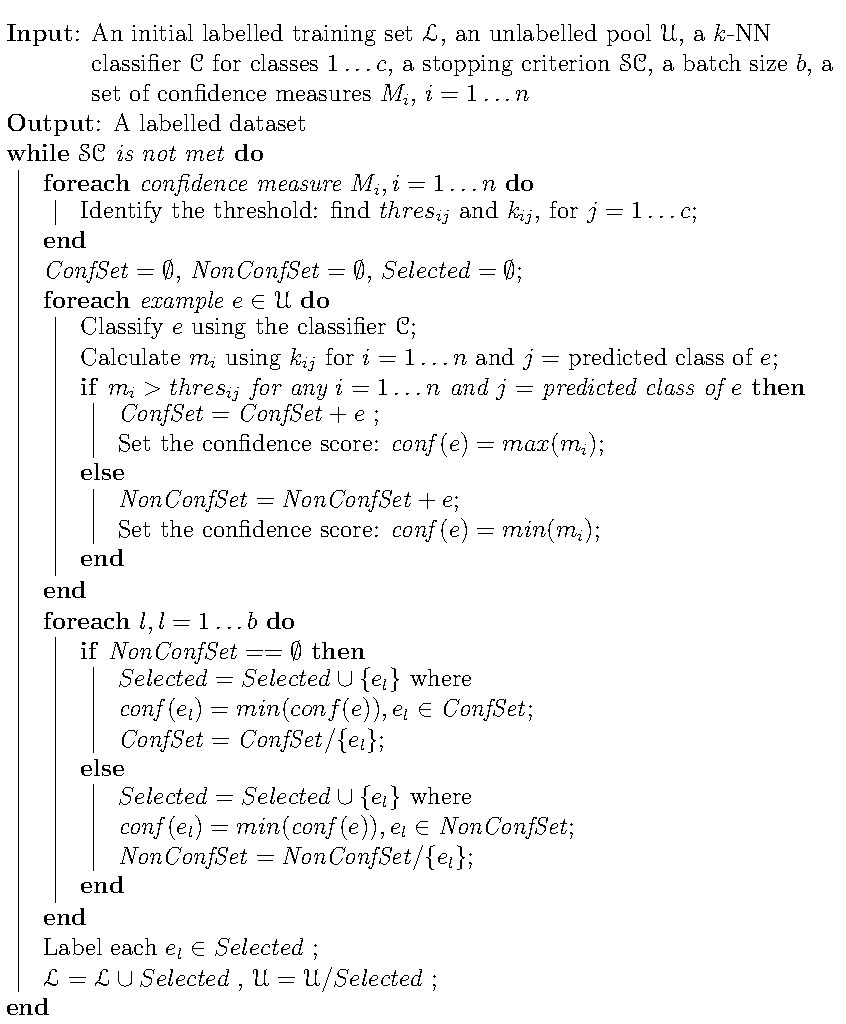
\includegraphics{./Others/Hu2011AggregrateAlgorithm}
\caption{Hu's Algorithm for the Aggregated Confidence Measures Selection Strategy}
\end{figure}

\subsection{Experiment Results}
Hu finds that using the aggregated confidence measure performs marginally (though not significantly) better than using any one of the confidence measures alone and also than Uncertainty Sampling.


\subsection{Comments}
I am unconvinced about the validity of the min-max style of aggregating the confidence measures.

The paper and thesis section seem rather unspecific about how the measures are normalised. I'm guessing there are broadly two possibilities :

\begin{enumerate}
	\item \textbf{Measure Threshold Normalization}
	
	In this case, measures would be normalized so that their thresholds would be the same.
	
	I don't think this was the case. If the thresholds alone were normalized, the measure ranges' maximum possible values would be different. As a result the maximum measure scores would definitely not be directly comparable.
	
	\item \textbf{Measure Range Normalization}
	
	In this case, the range of values over which the measure falls is normalized - giving the same minimum and maximum value possible for each measure. I don't think the measure threshold could then also be normalized, leading to different measures very likely having different thresholds. 
	
	If any measures pass their respective thresholds though, the maximum measure's value is chosen as the case's score, but this score may have nothing to do with the measure that actually caused the case to fail to be classed as confident. Scores are subsequently compared with other scores
	
	e.g. for a given class, 
	\begin{itemize}
		\item $thres(M1) = 0.8$
		\item $thres(M2) = 0.2$
	\end{itemize}
	and for a given case $case_{1}$ for that class:
	\begin{itemize}
		\item $m1 = 0.7$
		\item $m2 = 0.3$
	\end{itemize}  
	
	Because $m2 > thres(M2)$, the case will be put in the Confident set, and as such, the maximum of the measures will be taken - $m1=0.7$. Really the confidence measure that passed the threshold was $m2$ with a value of $0.3$.
	
	Now, imagine a different case $case_{2}$, but for the same class as above\footnote{The reason I'm specifying the same class is just to emphasize that the same thresholds apply. If it were a different class, different thresholds may apply - since thresholds are on a class-by-class basis - thus adding unnecessary complication to the example.}:
	\begin{itemize}
		\item $m1 = 0.1$
		\item $m2 = 0.6$
	\end{itemize}
	Again, because $m2 > thres(M2)$, the case will be put in the Confident set, but the maximum measure will be $m2 = 0.6$. 
	
	$case_{1}$ (with a score of $0.7$) will be treated as more \emph{confident} than $case_{2}$ (which has a score of $0.6$), even though $case_{2}$ was actually more confident than $case_{1}$ in the measure that actually caused it to be confident ($M2$).
	
\end{enumerate}

Whichever was the actual case - both seem flawed. The underlying fact remains that the different confidence measures aren't directly comparable, and the relatively simplistic manner in which the presented Aggregation Strategy deals with them - simply taking the maximum of all of them when any one is confident - does not appear to take this into account. Similarly with taking the minimum for the non-confident set.

It's possible there was some fancy-maths way to do the normalization which might hope to account for both range and threshold normalization, but I can't see how it could change the fact that a score is being assigned based on possibly a different confidence measure than the one which actually achieved confidence.

As a result of the above, we decided not to proceed with using Hu's aggregation strategy.

%TODO I'm not sure you're presenting this two systems clearly enough. Perhabs stand best out an overview - the intuition, then the algirhtm. Then dive in the details (formulae), and (culture?) these.

\chapter{Platform Architecture\label{cha:platarch}}
\section{Overview}
\subsection{Purpose}
The purpose of the system is the allow evaluation of and comparison between different Selection Strategies in a Pool-Based learning context.

It achieves this by executing each of the Selection Strategies on several data sets from an initially empty Case Base. At each Selection Strategy Selection, it runs a KNN based Classifier on the Case Base, evaluating its capability to correctly classify the instances in a test set.

\subsection{Technologies}
Weka\cite{prog:weka}, a Java based Machine Learning framework, was initially briefly investigated, but due to my familiarity with Python, Orange\cite{prog:orange} was used as the core Machine Learning component. It provided useful facilities to quickly get a basic evaluation platform up and running. As the platform progressed, most Orange dependencies were removed in favour of custom implementations due to the need for greater control, and a memory-management related bug which existed in Orange with regards its Python bindings for its C++ backend. Orange was subsequently just used for data loading, and distance computations.

For plotting, matplotlib\cite{prog:matplotlib} was initially used, but due to its very non-pythonic interface, we changed to using PyX\cite{prog:pyx}, which also provided much better support for LaTeX style file formats.

\section{Inputs}
\subsection{Data Files}
Data Files provide a table of instances, each instance consisting of attributes and a label. Orange provides support for loading many common formats, and also is capable of performing distance computation between instances based on their attributes.

For ease, Orange was used to perform initial data loading, and distance computation between instances. The instances, and the pair-wise distances were then serialized to a new data file to allow running on platforms (and runtimes) for which Orange wasn't present.

\subsubsection{Orange Supported}
Orange's primary data format is that of tabular, delimited text - such as CSV or TSV. Optionally, markup can be placed in the header rows of these files to help Orange know of the properties of each of the attributes - e.g. if the attribute represents the label for the instance, if the attribute is Discrete or Continuous, etc., but Orange is surprisingly good at figuring most of it out on its own - occasionally just needing slight nudging in the right direction.

Orange also supports some of the formats commonly used in other Machine Learning platforms - e.g. ARFF (as found in Weka) and correctly formatted .names, .data file pairs as sometimes found in the UCI Machine Learning Repository\cite{web:uci}\footnote{It should be noted that the majority of .data/.name pairs are not in the strict format necessary, thus some prior manipulation of the files present there may be needed to load them with Orange.}.

\subsubsection{Custom Pre-computed Distance Format}

The $n \times n$ distance matrix for a data-set can really be stored in a Symmetrical Matrix\footnote{This is assuming that the distance function is in fact symmetric, i.e. $d(a, b)\equiv d(b, a)$. In our distance function, this property does hold.}. Thus, when storing the distances for all pairs in the file, the space may essentially be halved by storing only one half of the $n \times n$ matrix\footnote{Technically, the distances between instances and themselves need not be stored, because by definition the distance between an instance and itself will be 0. Though this minor optimization is not performed in my code}.

\medskip

\begin{tabular}{ c c c c c c }
	Instance ID & \multicolumn{5}{c}{Distances} \\
	0 & $d(i_{0},i_{0})$ &  &  &  & \\
	1 & $d(i_{1},i_{0})$ & $d(i_{1},i_{1})$ &  &  &  \\
	2 & $d(i_{2},i_{0})$ & $d(i_{2},i_{1})$ & $d(i_{2},i_{2})$ &  & \\ 
	... & ... & ... & ... & ... & \\ 
	j & $d(i_{j},i_{0})$ & $d(i_{j},i_{1})$ & $d(i_{j},i_{2})$ & ... & $d(i_{j},i_{j})$ \\ 
\end{tabular}

\medskip

In addition to storing the distances, the label and a textual human-readable Payload/Instance Descriptor is also stored along with each Instance ID.

\paragraph{CSV}
The initial file type used for storing the precomputed distances along with the data was CSV (Comma Separated Values). The first line contains a header row. Subsequent lines contain the data rows. The first data row represents instance ID 0, the second represents instance ID 1, and so on. Each data row is organized as follows, where distances are stored in $n \times n$ matrix as described above:
\medskip

\begin{tabular}{ |c| |c| |c| }
	Textual Instance Description & Instance Label & Distances \\
\end{tabular}

\medskip

These files may also be gzipped - resulting in an extension .csv.gz, and this will be automatically uncompressed by the platform. The reason support for compression was added was due to the large file-sizes that resulted from the textual representation of the distances.

CSV was chosen due to it being quite trivial to produce irrespective of the programming language. It also allowed for easy debugging, and would also potentially allow other Machine Learning systems to be used for distance computation.

\paragraph{Google's Protocol Buffers\cite{prog:protocolbuffers}}

Google's blurb for Protocol Buffers is ``think XML, but smaller, faster, and simpler''\cite{prog:protocolbuffers}. It is binary format for which a proxy can be automatically generated for Python (among many other languages). It is used as the preferred method of loading data with precomputed distances in the presented platform, due to its compact representation, and efficient loading.

These files store essentially the same information in a similar method as the CSV style presented above. The devised protocol specification is as follows:
\begin{verbatim}
message Instance{
    optional string payload = 1;
    required string label = 2;
  }

message PrecomputedDistanceData{
  optional string data_set_name = 1;
  optional string data_set_description = 2;
  
  message Entry {
    required Instance instance = 1;
    repeated double distances = 2 [packed=true];
  }
  
  repeated Entry entry = 3;
}
\end{verbatim}

Most bits to the protocol are self explanatory. The number following each field is simply the field ID. In the Protocol Buffers specification, each field must have an integer ID, with each ID unique within its local namespace. The ``[packed=true]'' section is simply an optimization that allows the Protocol Buffers engine store the repeated numeric values in as compact a representation as it can.


\subsection{Experiment Definitions}
The definitions for the experiments to run need to be provided to the platform. Each experiment instance consists of data\footnote{ The data is provided as (training set, test set) pairs to allow for Cross-Validation, etc.} and the Selection Strategies to run on the data.

\subsection{Existing Results}
Existing results for Selection Strategies executed on the Data may also optionally be provided with the Experiment. When the Experiment is being executed, if it can find the results for a Selection Strategy within the provided existing results, these will be used as opposed to re-running that Selection Strategy again.

This allows for new Selection Strategies to be added and run, without re-computing previous strategies, but still having all outputs such as plots include the previous strategies' results.

It also allows for the graphs, etc. to be generated separately from the main experiment running\footnote{This can be useful, as then all the plotting/graphing dependencies need not be installed on all machines/platforms the experiment is being executed on.}, and due to ease of re-combining existing results, allows the experiment to be split, and different Selection Strategies be evaluated on separate machines concurrently.

\section{Experiment Execution}

\subsection{Selection Strategy Evaluation}
\subsubsection{Overview}
In Selection Strategy evaluation, the purpose is to execute a Selection Strategy against unlabelled training data\footnote{It's not really unlabelled - it's just from the perspective of the Selection Strategy it's unlabelled.}, to choose instances from the set and put them in the Case Base until the Stopping Condition is satisfied.

After each Selection, a KNN based classifier is given the Case Base as training data, and run on the test set, and the Classification Accuracy recorded.

The motivation is to judge how good each Selection Strategy is at selecting instances to maximize the ability of the Case Base to classify unseen instances.

\subsubsection{Selection Strategy}

A Selection Strategy in the platform is responsible for selecting instances to consult the Oracle for, given knowledge of what is already in the Case Base, and a pool of unlabelled instances to select from.

\subsubsection{KNN Classifier}
A K Nearest Neighbours based Classifier is used in the evaluation, with 
\begin{itemize}
	\item $k=5$\footnote{This was indeed arbitrary - it simply being an apparently relatively common k to use in the literature. Due to distance weighted voting being used - it isn't really of much importance.} 
	\item Euclidean Distance after Attribute Normalization\footnote {This functionality was provided entirely by Orange.}
	\item Distance Weighted Voting. The distance function used is:
	
	\[
	\frac{1}{distance^{2}+10^{-10}}
	\]
	
	where $distance$ is normalized between $0$ and $1$, and the $10^{-10}$ is simply to account for $distance$ being $0$, giving a high weighting to when this happens.
	
	
\end{itemize}

An overview of KNN Classification can be found online.\cite{web:knntut}.

\subsubsection{Cross Validation}

10-Fold Cross Validation is used for training/testing against the data. Initially Orange was used to provide Stratified Folds, but later, during the Orange-dependency-removal stage - a simplistic non-stratified implementation was adapted from the SciKit Learn library\cite{prog:sklearn}.

Many walkthroughs of K-Fold Cross Validation exist online\cite{web:kfolddemo}, but the basic approach is to split the data into k sets, followed by iteratively choosing one of the sets as the test set, and the union of the remaining sets as the training set. Thus, the testing is repeated k times. The results of the k tests are then averaged to produce a single result.

\subsubsection{Basic Evaluation Algorithm}
\begin{samepage}
\begin{verbatim}
let result_sets = {}
for each (training_set, test_set) in the CV Sets:
  let unlabelled_set = training_set
  let case_base = {}
  let result_set = {}
  while the stopping criteria is not met:
    let selections = select instances from the 
                     unlabelled_set using the 
                     selection strategy.
    ask oracle for labels for all of selections
    remove the selection from unlabelled_set
    add selections to case_base with their label
  
    let result = Result from testing the classifier
                 built using case_base on test_set
    add result to result_set
  add result_set to result_sets
\end{verbatim}
\end{samepage}

\subsection{Experiment Outcome Representation}
\subsubsection{Result}
An individual result consists of:
\begin{itemize}
	\item Size of the Case Base
	\item Classification Accuracy of the Case Base
	\item Selections from the Selection Strategy that were just added.
\end{itemize}

\subsubsection{Result Set}
A Collection of Results, which also provides the capability to generate the AULC of the results. For convenience and completeness, a Result Set also has knowledge of the Training Set and the Test Set that was used in generating the contained Results.

\subsubsection{Multi Result Set}
A collection of Result Sets, which provides averaging of Results grouped by Case Base size, which can subsequently act as a standard Result Set based on the averaged results.

\subsection{Summarising The Results}
\subsubsection{Learning Curve}\label{sec:multiresultset}
A commonly presented representation of Selection Strategy Evaluation is the Learning Curve - a plot of Classification Accuracy vs Case Base Size.

\subsubsection{Area Under the Learning Curve}
A metric to summarise the progression, and allow for comparison among different Selection Strategies against the same data set and same starting and finishing Case Base size is AULC (Area Under the Learning Curve). As can be expected, this is simply the area under the Learning Curve.

\section{Outputs}

\subsection{Raw Selection Strategy Results}
The primary and non-optional outputs of the platform are the raw Selection Strategy results for all the provided data sets. From these, the other outputs can be calculated. It is also these raw results which can be provided to another run of an experiment so that they need not be re-computed if they are needed by the experiment. 

For space efficiency, and ease of manipulation, each set of Selection Strategy results for a data set are stored in a compressed archive.

These Raw Results represent the Serialized form of a Multi Result Set as presented on page \pageref{sec:multiresultset}. When the Raw Results are provided to the program, it is to a Multi Result Set it is Deserialized to.

\subsubsection{Individual Cross Validation Results}
For each data-set and subsequently for each Selection Strategy - the evaluation on each Selection Strategy is carried out multiple times due to the k-Fold Cross Validation Methodology used. As such, there will be k different sets of results. 

Within the compressed Selection Strategy Results Archive, these are labelled 0.csv, 1.csv, etc. with each corresponding to the fold number in the Cross Validation splits of the data set.

Each csv contains essentially 3 items. \footnote{The format of these 3 items is somewhat hacky, and was went for purely in laziness. Splitting into separate files would have added unnecessary complexity when so many other aspects of the project needed time.}

\begin{enumerate}
	\item Results for various Case Base sizes, with each Result instance denoted with:
		\begin{itemize}
			\item The Case Base Size
			\item The Classification Accuracy
			\item The list of Selections that were made by the Selection Strategy just prior to this test.
		\end{itemize}
	\item The Training Set used for this Cross Validation
	\item The Test Set used for this Cross Validation
\end{enumerate}

\subsubsection{Summary Results}
Summary Results are also saved\footnote{Technically, these Summary Results are unnecessary, as they can simply be recomputed using the raw individual Cross Validation Results. They are simply there for user ease.}, and are similar to the CSV style of Raw Cross Validation Results except do not contain lists of Selections, or the Test Set or Training Set, but are in a file named ``summary.csv''.

\subsection{Learning Curve Plots}
PyX\cite{prog:pyx} is used to generate a PDF file of plots of the Average Learning Curves for all of the Selection Strategies\footnote{Initially - matplotlib\cite{prog:matplotlib} was used to generate the graphs - but its interface was somewhat messy and non-pythonic.}. One PDF is generated for each Data Set.

\subsection{Selection Graphs}
Node/Edge style graphs are also generated for each of the Selection Strategies. The distance matrix for the entire Data Set is used to generate a Spring-graph of all the instances, where each instance has an edge to its 5 Nearest Neighbours, with a force proportional to the distance. Graphviz\cite{prog:graphviz} was used to perform this graph generation, with PyGraphviz\cite{prog:pygraphviz} as the interface to Python.

Instances which a given Selection Strategy chooses are highlighted at each Selection iteration. These are then output to a PDF file, with each page representing an iteration in the Selection Strategy.

Because Selections can't really be averaged across the different Folds in the Cross Validation, a PDF file is generated for each Cross Validation fold. Grey Nodes represent Test Instances, Black Nodes represent Unlabelled Instances, and Green Nodes represent Nodes selected by the Selection Strategy.

Due to the flattening of varying dimensionality Data Sets, the usefulness of these graphs vary widely depending on the Data Sets used, so it is not useful in all instances.

\subsection{Experiments Summary}
A summary CSV file is also output for the Experiments executed during a run of the platform. It simply gives tabular breakdown of Data Set vs Selection Strategy of AULC values.

\chapter{Competence Models\label{cha:CompetenceModels}}
\section{Overview}

Delaney, in her work, expanded upon the definitions of Coverage and Reachability sets to include their counterparts, what she terms ``Liability'' and ``Dissimilarity'' respectively \cite{Delany2009}. She subsequently uses these concepts in defining Case Profiles, which she uses Case Base Maintenance strategies.

From Delaney's work, we hope to expand on her boolean RCDL Profile concepts, and attempt to use them in an Active Learning Selection Strategy role.

This chapter first outlines the fundamental concepts involved in RCDL profiles as presented by Delaney, and subsequently expands on these to describe how we use them in our Selection Strategy context.

\section{Fundamentals}
\subsection{Classifies / Misclassifies}
\subsubsection{Case Contribution\label{sec:contributes}}
Both Classifies and Misclassifies are subsequently defined in terms of \emph{Case Contribution}.

A case $c$ contributes to another case $c'$'s classification if $c$ is retrieved as a nearest neighbour of $c'$ and $c$ aids 'positively' to $c'$'s classification (i.e. is the same class as $c'$ if $c'$ is correctly, or is a different class to  $c'$ if  $c'$ is incorrectly classified).
\subsubsection{Classifies}
\begin{quote}
$ Classifies(t, c) $ means that case c contributes to the correct classification of target case t. This means that target case t is successfully classified and case c is returned as a nearest neighbour of case t and has the same classification as case t.\cite{Delany2009}
\end{quote}

Therefore, for $ Classifies(t, c) $:
\begin{enumerate}
	\item t must be correctly classified by the case base.
	\item c must be returned as a NN of t in that correct classification.
	\item c must be of the same class as t.
\end{enumerate}

\subsubsection{Misclassifies}

\begin{quote}
$ Misclassifies(t, c ) $ means that case c contributes in some way to the incorrect classification of target case t. In effect this means that when target case t is misclassified by the case-base, case c is returned as a neighbour of t but has a different classification to case t.\cite{Delany2009}
\end{quote}


Therefore, for $ Misclassifies(t, c) $:
\begin{enumerate}
	\item t must be incorrectly classified by the case base.
	\item c must be returned as a NN of t in that classification.
	\item c must be of a different class than t's actual class.
\end{enumerate}

\subsubsection{Example}
\begin{figure}[h!]
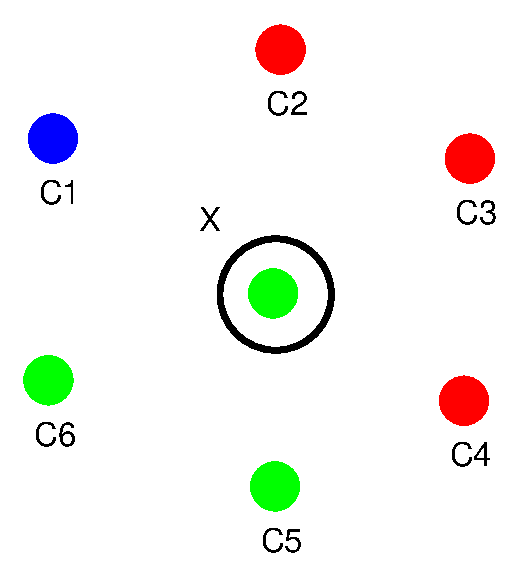
\includegraphics[width=5cm]{./Drawn/EqualDistanceMisclassifiesEg}
\end{figure}

e.g  in the above example, the circled case $x$ is incorrectly classified as red by the case base (with k=6). Here, the 3 reds (c2, c3 and c4) and the 1 blue (c1) contribute to the incorrect classification, and thus:
\begin{itemize}
	\item $ Misclassifies(x, c1) $
	\item $ Misclassifies(x, c2) $
	\item $ Misclassifies(x, c3) $
	\item $ Misclassifies(x, c4) $
\end{itemize}

\subsection{Nearest Neighbours / Reverse Nearest Neighbours}
Before considering the definitions of the RCDL sets, it is useful to consider the notion of nearest neighbours and reverse nearest neighbours, so that the RCDL sets can be framed in those terms.

\subsubsection{Nearest Neighbours (NNs)}
For a case c, $ NNs(c) $ is the set of cases within the k nearest neighbours of c, excluding c itself.

\subsubsection{Reverse Nearest Neighbours (rNNs)}
For a case c, $ rNNs(c) $ is the set of cases that have c in their NNs set.

\subsubsection{Example}
\begin{figure}[h!]
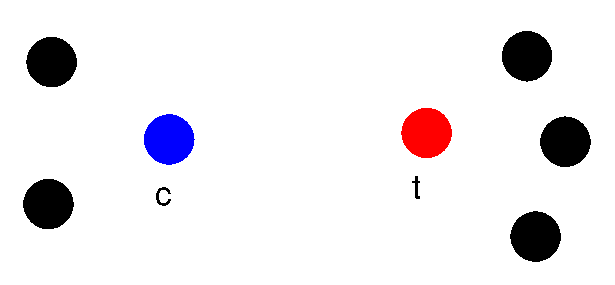
\includegraphics[width=5cm]{./Drawn/RcdlNnRnnEg}
\end{figure}

For $k=3$:
\begin{itemize}
	\item $ t \in NNs(c) $
	\item $ c \in rNNs(t) $
\end{itemize}

\subsection{RCDL Definitions}
Overall Reachability and Coverage relate to cases being correctly classified by the case base, whereas Dissimilarity and Liability relate to cases being incorrectly classified by the case base.

Reachability and Dissimilarity are concerned with the neighbouring cases of a case, whereas Coverage and Liability are concerned with the cases to which a case is a neighbour.

\subsubsection{Reachability Set}
\[ ReachabilitySet(c \in C) = \left\lbrace t \in C : Classifies(c, t) \right\rbrace \] 
If c is correctly classified by the case base, these are all the cases in $ NNs(c) $ that have the same class as c. Otherwise, this set is empty (and the Dissimilarity set is instead populated).

\subsubsection{Coverage Set}
\[ CoverageSet(c \in C) = \left\lbrace t \in C : Classifies(t, c) \right\rbrace \]
These are all the cases $ t \in rNNs(c) $ such that t is correctly classified by the case base and the class of t is the same as the class of c.

\subsubsection{Dissimilarity Set}
\[ DissimilaritySet(c \in C) = \left\lbrace t \in C : Misclassifies(c, t) \right\rbrace \]  
If c is incorrectly classified by the case base, these are all the cases in $ NNs(c) $ that have a different class than the actual class of c. Otherwise, this set is empty (and the reachability set is instead populated).

\subsubsection{Liability Set}
\[ LiabilitySet(c \in C) = \left\lbrace t \in C : Misclassifies(t, c) \right\rbrace \]  
These are all the cases $ t \in rNNs(c) $ such that t is incorrectly classified by the case base, and the class of c is different from the class of t.

\section{Delaney's Analysis}

\subsection{Case Classifications}
Through the definitions of the RCDL Sets - Delaney notes the following\cite{Delany2009}\footnote{The two enumerations following of profile analysis are taken verbatim from the cited paper. They gives a good break-down of the possibilities, and are simply useful to keep in mind when considering the rest of the RCDL approach - hence their inclusion.}:

\begin{enumerate}
	\item Firstly, it is possible to indicate whether the case is correctly or incorrectly classified by the case-base. This is identified by the case having either a reachability set (R) or a dissimilarity set (D).
	\item Secondly, we can consider whether the case is useful, by the existence of a coverage set (C), and
	\item Finally whether the case is harmful and causes damage, by the existence of a liability set (L).
\end{enumerate}

Through enumeration of the possible RCDL Combinations - 8 possible Profiles exist for a case, using the occurrence of a non-empty set as the \emph{flag} on which to enumerate\cite{Delany2009}:

\begin{enumerate}
	\item \emph{R}: A case which is correctly classified but is not used for classifying any other case in the case-base.
	\item \emph{D}: A case which is misclassified but is not used for classifying any other case in the case-base.
	\item \emph{RC}: A case which is correctly classified and is useful in that it has contributed to the correct classification of other cases in the case-base. This profile and the R profile are generally the majority case profile types.
	\item \emph{RL}: A case which is correctly classified but is harmful in the case-base causing damage by contributing to other cases being misclassified.
	\item \emph{DC}: A case which is misclassified but is useful in the case-base. 
	\item \emph{DL}: A case which is misclassified and is harmful in the case-base.
	\item \emph{RCL}: A case which is correctly classified and is both useful and harmful in the case-base.
	\item \emph{DCL}: A case which is misclassified and is both useful and harmful in the case-base.
\end{enumerate}


\subsection{Experimental Conclusions}
In her experiments, Delaney investigates the effect on case base competence of removing cases with different combinations of RCDL profiles. She also compares the strategies with other Noise-removal strategies, and frames them in RCDL terms.

While the specific results vary between datasets, Delaney notes that there was a consistent improvement with the removal of just DL \& DCL cases from the datasets. 

The reader is recommended to consult \citet{Delany2009} for the thorough analysis.

\section{Continuing From Delaney's Work}
The simplicity of the boolean set-non-emptiness characteristic of the case profiles Delaney defines has its serious merits. It is relatively easy to understand and reason about. 

Though it does throw away much potentially useful information. It does not try to do any reasoning about the contents of the set

In our work, we hope to play with further expanding on these profiles - using them in a non-boolean way, instead factoring in what the sets actually comprise of.

\section{RCDL Consequences}

\subsection{Either-or nature of Reachability and Dissimilarity Sets}
If a case has a non empty reachability set then it has been classified correctly by the case-base and, as such, will have an empty dissimilarity set and vice versa.

Intuitively – these sets simply represent the set of cases that contribute to a case's classification (with the notion of \emph{contributes} as outlined above on page \pageref{sec:contributes}). 

If the case is correctly classified, this set is said to be the Reachability set, whereas if incorrectly classified, it is termed the Dissimilarity set.

\subsection{Reachability-Coverage / Liability-Dissimilarity Duality}
Simply put, if case $c$ occurs in case $t$'s Reachability set, case $t$ occurs in $c$'s Coverage set. Similarly with Liability and Dissimilarity.
The reasoning is as follows:
\begin{itemize}
	\item Take a single case pair, $c1$ and $c2$ such that $Classifies(c1, c2)$.
	\begin{itemize}
		\item $c2$ contributes to the correct classification of $c1$.
	\end{itemize}
	\item From $c2$'s perspective, $c1$ is in its Coverage set.
	\begin{itemize}
		\item From the formula above, from $c2$'s perspective, $c=c2$, and $t=c1$, and it is the case that $Classifies(t, c)$.
	\end{itemize}
	\item From $c1$'s perspective, $c2$ is in its Reachability set.
	\begin{itemize}
		\item From the formula above, from $c1$'s perspective, $c=c1$ and $t=c2$, and it is the case that $Classifies(t, c)$.
	\end{itemize}
\end{itemize}

Similar reasoning can be applied to the Liability and Dissimilarity sets.

This point is easier to understand just by intuition around the plain-English definitions of the RCDL profiles above.

\subsection{Reachability is to Dissimilarity as Coverage is to Liability}
This is obvious from looking at the formulas, but is worth pointing out for future notes.

\subsection{Reachability/Dissimilarity concerned with Nearest Neighbours, Coverage/Liability with Reverse Nearest Neighbours \label{sec:RdWithNnClWithRnn}}
This can simply be derived through the definitions above, but of primary note is that:
\begin{itemize}
	\item The Reachability and Dissimilarity of a case can be inferred by just looking at that case's nearest neighbours
	\item The Coverage and Liability of a case can be inferred by just looking at that case's reverse nearest neighbours (assuming the case-base classification of each of the reverse nearest neighbours is known)
\end{itemize}

\subsection{Max Size of Reachability and Dissimilarity Sets bounded to K}
Given that the Reachability and Dissimilarity of a case are always subsets of that case's NNs, the maximum size is the size of the NNs set – K. (This is assuming that a \emph{strict} kNN is used, where at max k neighbours are used even when ties exist).

\section{An Incremental Strategy to RCDL}
\subsection{Justification} 
In Delaney's work, it was sufficient to calculate the Case Base RCDL profiles in a brute-force manner, since it was the most efficient way for use in her Case Base Maintenance investigation on existing Case Bases. In our case for Selection Strategies, this would not be the case, since the profiles would be need to be inferred many times for a changing Case Base.

It would also be useful to be able to determine what RCDL changes would occur in the RCDL profiles if a new case was added with a given class. If this were to be done for each unlabelled case when selecting a case to add to the case base, it would be very expensive to re-build the entire set of RCDL profiles for the case base each time.

Thus, we decided to create an incremental strategy, in which the changes can also be inferred in linear time before actually \emph{adding} a case.

\subsection{Desired Algorithm Structure}
\subsubsection{Inputs}
\begin{itemize}
	\item A case base 
	\item k – the size of the neighbourhood
	\item RCDL, NN, and rNN profiles for each of the cases
\end{itemize}

For the remainder of this algorithm description, the term `profile' is used to denote the RCDL profile plus NNs plus rNNs. i.e. 
\begin{verbatim}
CaseProfile:  
  Reachability Set:  {…}
  Coverage Set:      {…}
  Dissimilarity Set: {…}
  Liability Set:     {…}
  NNs:               {…}
  rNNs:              {…}
\end{verbatim}

\subsubsection{Operations}
\paragraph{$Suppose(unlabelled\_case, class)$}
This operation should determine what changes would occur to the profiles of the cases in the case base if a given unlabelled case was added to the case base, with a given class.

A Change to a given case may be denoted as the pair (Added, Removed), where Added and Removed in turn are simply partial profiles. i.e.
\begin{verbatim}
Change:
  Added:
    Reachability Set:  {…}
    Coverage Set:      {…}
    Dissimilarity Set: {…}
    Liability Set:     {…}
    NNs:               {…}
    rNNs:              {…}
  Removed:
    Reachability Set:  {…}
    Coverage Set:      {…}
    Dissimilarity Set: {…}
    Liability Set:     {…}
    NNs:               {…}
    rNNs:              {…}
\end{verbatim}

The output for this algorithm will be a set of (Case, Change) pairs. For algorithmic ease, this also include the input unlabelled case, since technically, adding it will cause cases to be added to its Reachability Set, etc. But understandably, for the input case's Change, the Removed data will always be empty.

\paragraph{$Add(labelled\_case)$}
This operation simply adds a given case to the case base, updating the case base's profiles as appropriate. Operationally, this involves supposing that the case was added with its class using the previous Suppose operation, and updating the case base's profiles as per the returned set of (case, Change) pairs.

\subsection{Algorithm Outline}
The rough approach taken is to first determine the changes which occurred to NNs and rNNs. From these, along with knowledge of the existing RCDL profiles, the changes to Reachability, Coverage, Dissimilarity and Liability are inferred. \footnote{Note – for clarity, the outline refers to updating the actual Case Base Profiles set, whereas really it's a Change object for each one that it modifies, and finally returns}

\subsubsection{Figuring out NN / rNN changes}
\paragraph{Notes}
\subparagraph{Determining if an existing case has the new case as a NN within k}
Unfortunately, each case in the case base needs to be examined to determine if it has the new case as a NN. But because we have the NNs stored for each case in the case base, the examination of each case can be a relatively quick operation (versus the alternative of having to, for each case, go through the entire case base to find its NNs if they weren't stored).

The maximum NN distance in the cached NN list need only be compared to the distance of the new case (with consideration for tie breaking as in the kNN classifier if they're equal).

\subparagraph{Get or create Change in all\_changes for x}
This is simply a shorthand for first checking if there already is a change in all\_changes for $x$, and if so, retrieving it – otherwise creating a new blank Change in all\_changes for $x$, and returning the new Change.

%TODO Not clear (too low level?)

\subparagraph{Duality of NN/rNN changes (both added and removed)}
If a case has a Nearest Neighbour added, then for that Nearest Neighbour, it will get a Reversed Nearest Neighbour added. Thus, for any NN add, there is a corresponding rNN add. Similarly for remove.


\paragraph{Algorithm}

\begin{samepage}
{\small 
\begin{verbatim}
// Sort out the new case's Nearest Neighbours
For each NN of the new case's NNs:
  add the new case to their rNNs

// Sort out the new case's Reverse Nearest Neighbours.
For each existing case that has the new case as a NN:
  Add the existing case to the new case's rNNs
  Add the new case to the existing case's NNs.
  If the new case shunted an NN of the existing case:
    Remove shunted case from the existing case's NNs
    Remove existing case from the shunted case's rNNs.
\end{verbatim}
}
\end{samepage}

\subsubsection{Using NN / rNN changes to determine RCDL changes}
\paragraph{Notes}
\subparagraph{Ability to just look at NN changes}
Due to the NN/rNN Duality property described above with regards NN changes, any NN add is guaranteed to have an rNN add, and similarly with remove. This allows us to consider only NN changes, and while dealing with the NN change, deal with the corresponding rNN change.

\subparagraph{Permutations of NN changes}
Because of the previous note, we only really need to deal with the added and removed nearest neighbours. So – the permutations of NN changes for a single case, following `supposing' the addition of a single case:

\medskip

\begin{tabular}{ | c | c | p{5cm} |} \hline
	NN Added & NN Removed & Notes \\ \hline
	1 & 1 & Will be the only type when the size of the case base is greater than or equal to  k. \\ \hline
	1 & 0 & Happens only at start, as the NN is filling to capacity. Same as added above. \\ \hline
	0 & 1 & Can never actually happen - would have to be another replace it. \\ \hline
	0 & 0 & Uninteresting - its rNNs will be covered elsewhere with the NN changes of another case. \\ \hline
\end{tabular}

\subparagraph{A NN Removal Guarantees an NN Add}
This can be seen in the truth table above. Because we're only dealing with a new case being added, the effect of the new case can never cause a NN removal without causing a corresponding NN add of the new case. (Because of having a shorter distance to the target case than the furthest-distance NN, the new case will have \emph{shunted} that NN – causing a NN removal).

This allows us to not worry about, at the stage of dealing with NN removals, if the removal caused the class to change, because we'll be dealing with that scenario anyway in the corresponding add.

\subparagraph{A NN removal might affect R/D of me, C/L of other}

\begin{figure}[h!]
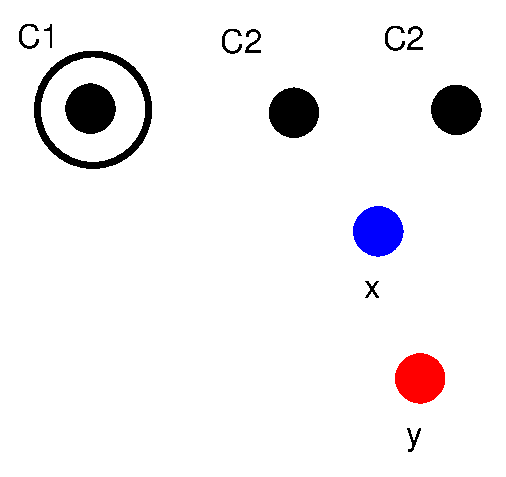
\includegraphics[width=5cm]{./Drawn/NnMightAffectEg}
\end{figure}


In the above example,
\begin{itemize}
	\item $k=3$, 
	\item $x$ is the case of interest whose NNs  we'll talk about
	\item $y$ is the new case added to the case base
	\item $c1$, $c2$, $c3$ are the NNs of $x$ prior to $y$ being added
	\item $c1$ is the \emph{shunted} case which is removed from NNs(x) after $y$ is added.
\end{itemize}

$c1$ was an NN of $x$, and $x$ was an rNN of $c1$. As described previously in \ref{sec:RdWithNnClWithRnn}, a case's NNs can affect its Reachability / Dissimilarity sets, whereas a case's rNNs can affect its Coverage / Liability sets. So the removal of $c1$ as an NN of $x$ (and the corresponding removal of $x$ as an rNN of $c1$) might affect $c1$'s Reachability / Dissimilarity set, and $x$'s Coverage / Liability set, because when $c1$ is removed as a NN, it can't contribute either positively or negatively any more to $x$'s classification.\footnote{Note that it is not guaranteed that $c1$ was in $x$'s Reachability / Dissimilarity set, or that, equivalently, $x$ was in $c1$'s Coverage / Liability set. The sets will only be affected if $c1$ was a \emph{contributor} of $x$'s classification by the case base. Hence the usage of ``might affect''.}

All this leads to a simple way to dealing with an NN removal \footnote{The corresponding NN addition will be dealt with separately}:
\begin{itemize}
	\item If $c1$ was in $x$'s Coverage / Liability set, it should be removed.
	\item If $x$ was in $c1$'s Reachability / Dissimilarity set, it should be removed.
\end{itemize}

\subparagraph{Calculating a case's new classification}
This can be done semi-intelligently since a case's old NNs are known. Instead of doing kNN classification with the entire case base, we only need to look at a case's new NNs (which can be inferred from its old NNs and the NN changes) to determine the new classification.

\subparagraph{Correct-classification-status}
We will furthermore commonly talk about a case's correct-classification-status as opposed to its classification alone. It simply means whether a case has been correctly classified by the case base or not. 

\subparagraph{A case's correct-classification-status determining Reachability/Dissimilarity}
If a case is correctly classified by the case base, its Reachability set will be populated. If it is incorrectly classified, its Dissimilarity set will be populated.
 
\subparagraph{Effect of a correct-classification-status changing}
Firstly, we need only worry about if the correct-classification-status of a case changes with the addition of a new case, as opposed to if the classification alone changes.

E.g. if a case's actual class was `green', it was previously classified `blue', and with the addition of the new case, it's classified `red', it has still been incorrectly classified both before and after the addition of the new case, therefore we do not need to worry about scrubbing.

If however the correct-classification-status of a case does change, we need to perform \emph{scrubbing} on some of the RCDL sets.

If it went from correctly classified to incorrectly classified:
\begin{itemize}
	\item The case's Reachability set needs to be scrubbed (all items removed).
	\item For each \emph{scrubbed} case from the Reachability set, the scrubbed case needs to have `case' removed from its Coverage set.
	\item The case's Dissimilarity set needs to be populated with the elements in its new NNs that have a different class to its actual class.
	\item For each thing put in the Dissimilarity set, their Liability sets need to have `case' added.
\end{itemize}

Similarly, if it went from incorrectly classified to correctly classified:
\begin{itemize}
	\item The case's Dissimilarity set needs to be scrubbed (all items removed).
	\item For each \emph{scrubbed} case from the Dissimilarity set, the scrubbed case needs to have `case' removed from its Liability set.
	\item The case's Reachability set needs to be populated with the elements in its new NNs that have the same class as its actual class.
	\item For each thing put in the Reachability set, their Coverage sets need to have `case' added.
\end{itemize}

%TODO I'm not sure this explanation is working. ie clear enough yet. Test: Could one of your (brighter) colleagues understand it?

\subparagraph{Not allowing supposing of an already present case}
The algorithm presented does not allow for an already present case in the case base to be \emph{supposed} (e.g. if x is in the case base with class `blue', what would happen if x was actually `red').

\subparagraph{Not allowing for supposing the removal of a case}
The algorithm presented does not allow for supposing the removal of a case from the case base (e.g. what would happen if I removed x from the case base?), though it could be updated to support this scenario.
 
\paragraph{Algorithm Outline}

\begin{samepage}
{\small 
\begin{verbatim}
Compute the NN/rNN changes using the suppose_nn algorithm.
foreach case in the NN/rNN changes:
  // Deal with NN removals, if present
  foreach removed_case in case's NN removals:
    if the removed_case was in case's Reachability set:
      Remove removed_case from case's Reachability set
      Remove case from removed_case's Coverage set.
    else if removed_case was in case's Dissimilarity set:
      Remove removed_case from case's Dissimilarity set
      Remove case from removed_case's Liability set.

  // Deal with NN adds, if present
  if no NN adds for case:
    jump to start of loop for next case

  Calculate case's new classification
  
  if the case's correct-classification-status changed:
    // Need to scrub appropriate RCDL sets
    for each r in the case's old `contributors' list:
      if the case's old classification was the correct:
        Remove r from case's Reachability set
        Remove case from r's Coverage set
      else:
        Remove r from case's Dissimilarity set
        Remove case from r's Liability set
  foreach c in the case's new `contributors' list:
    if the case's new classification is correct:
      Add c to case's Reachability set
      Add case to c's Coverage set
    else:
      Add c to case's Dissimilarity set
      Add case to c's Liability set

\end{verbatim}
}
\end{samepage}
\subsection{Testing and Validation}

\section{Competence Based Selection Strategies}
\chapter{Experimental Analysis\label{cha:expanalysis}}
\section{Datasets Used}
\subsection{Non-Textual}
\subsubsection*{Breathalyzer}\label{sec:breathalyzer}
\subsubsection*{Dermatology}\label{sec:dermatology}
\subsubsection*{Glass}\label{sec:glass}
\subsubsection*{Haberman}\label{sec:haberman}
\subsubsection*{Heart Disease}\label{sec:heart_disease}
\subsubsection*{Hepatitis}\label{sec:hepatitis}
\subsubsection*{Iris}\label{sec:iris}
\subsubsection*{Lung Cancer}\label{sec:lung_cancer}
\subsubsection*{TA Evaluation}\label{sec:taevaluation}
\subsubsection*{Wine}\label{sec:wine}
\subsubsection*{Zoo}\label{sec:zoo}
\subsection{Textual}

\section{Basic Selection Strategies}


\section{Competence-based Selection Strategies}

\section{Results}
Results are presented using a learning curve (Accuracy vs Case-Base Size). The AULC figure is also calculated.

\subsection{Non-Textual Datasets}

\begin{figure}[h!]
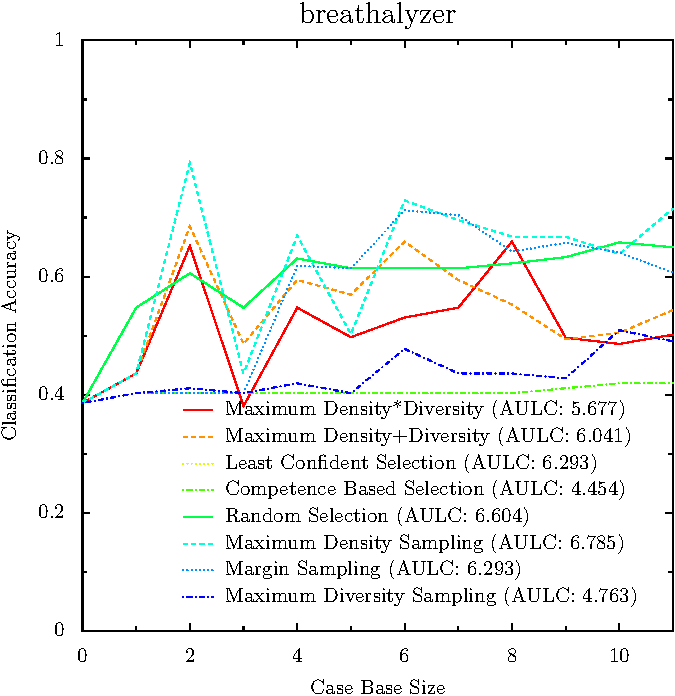
\includegraphics{./Plots/breathalyzer}
\caption{Learning Curve Plots for `Breathalyzer' Dataset (\ref{sec:breathalyzer})}
\end{figure}

\begin{figure}[h!]
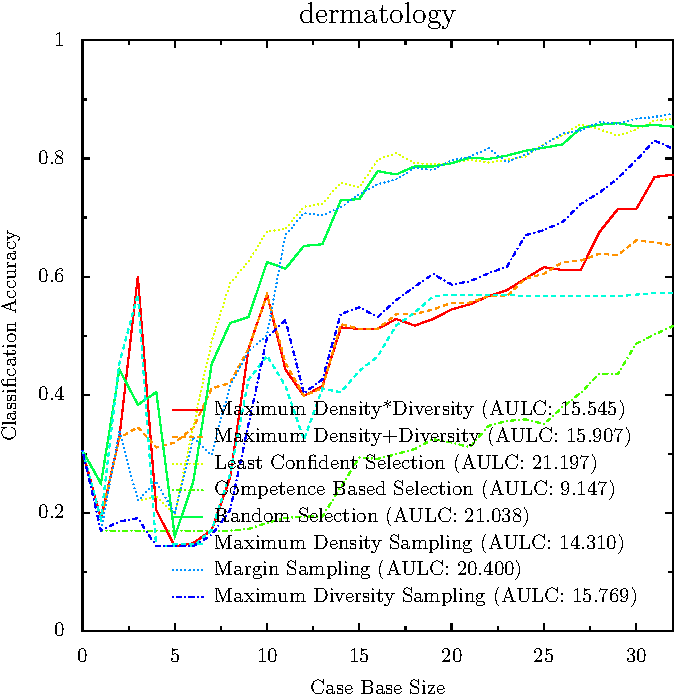
\includegraphics{./Plots/dermatology}
\caption{Learning Curve Plots for `Dermatology' Dataset (\ref{sec:dermatology})}
\end{figure}

\begin{figure}[h!]
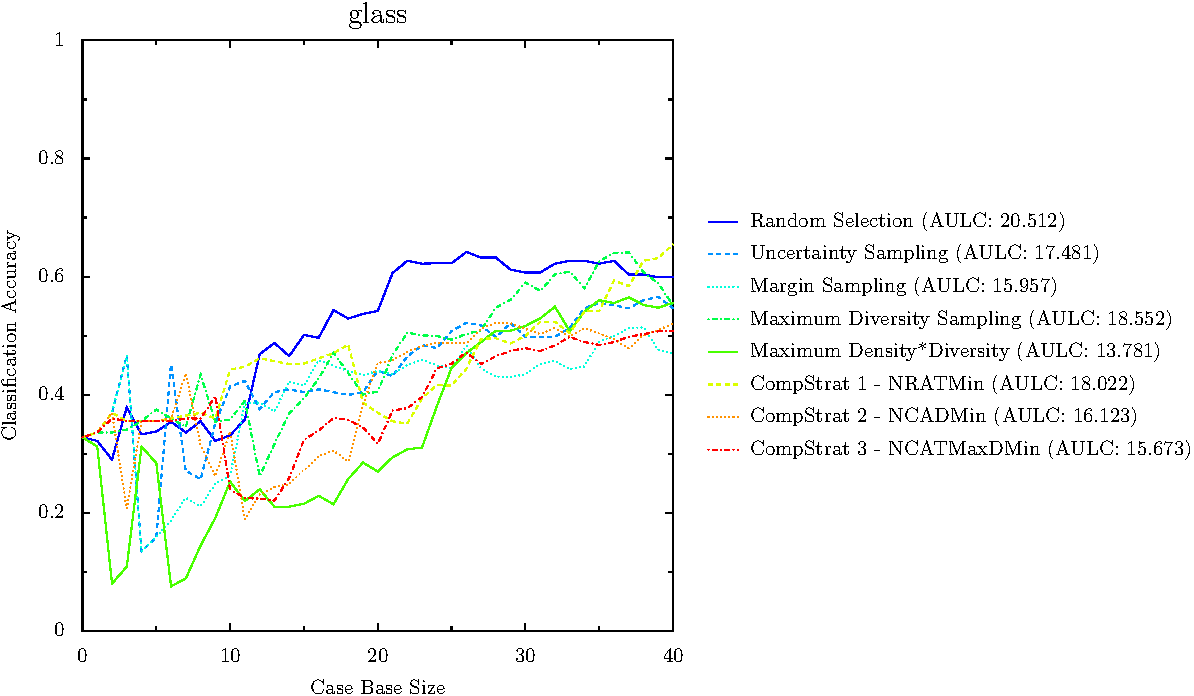
\includegraphics{./Plots/glass}
\caption{Learning Curve Plots for `Glass' Dataset (\ref{sec:glass})}
\end{figure}

\begin{figure}[h!]
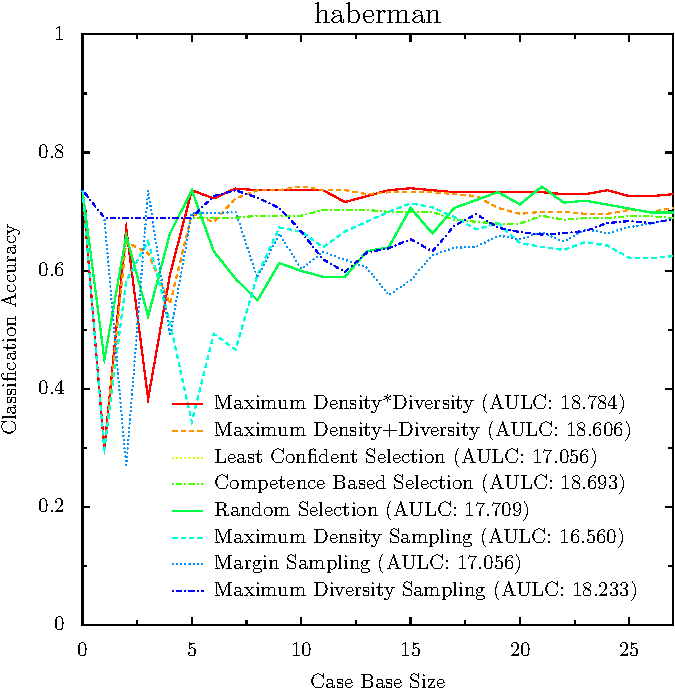
\includegraphics{./Plots/haberman}
\caption{Learning Curve Plots for `Haberman' Dataset (\ref{sec:haberman})}
\end{figure}

\begin{figure}[h!]
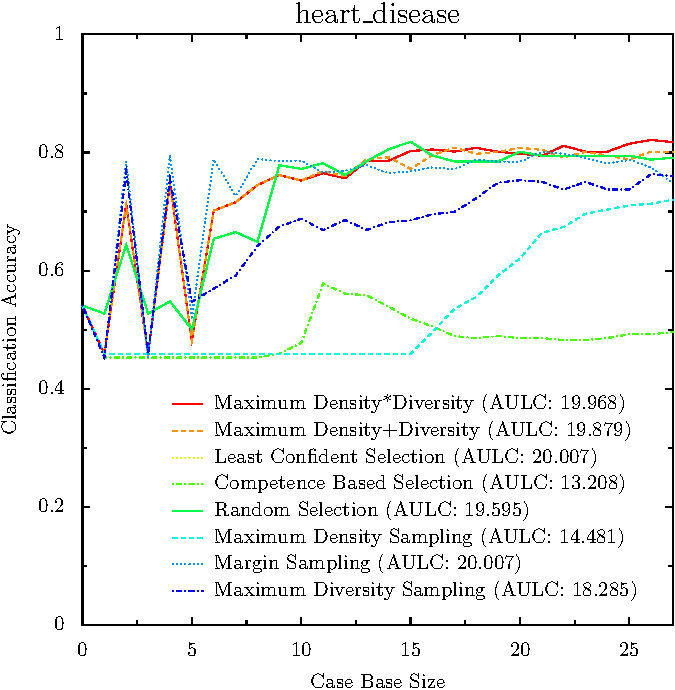
\includegraphics{./Plots/heart_disease}
\caption{Learning Curve Plots for `Heart Disease' Dataset (\ref{sec:heart_disease})}
\end{figure}

\begin{figure}[h!]
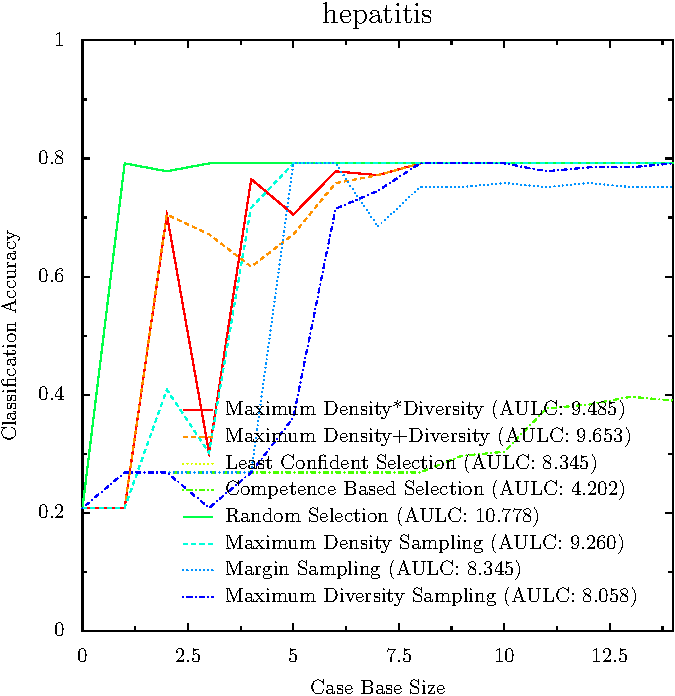
\includegraphics{./Plots/hepatitis}
\caption{Learning Curve Plots for `Hepatitis' Dataset (\ref{sec:hepatitis})}
\end{figure}

\begin{figure}[h!]
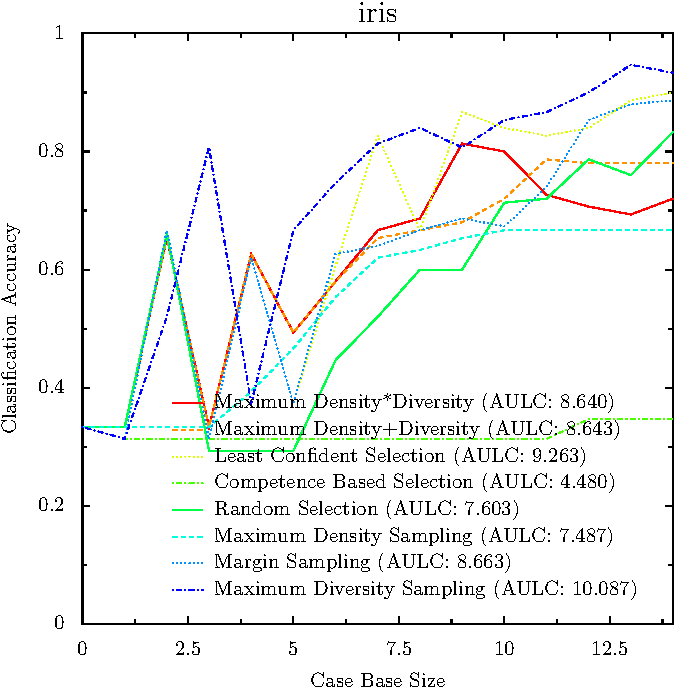
\includegraphics{./Plots/iris}
\caption{Learning Curve Plots for `Iris' Dataset (\ref{sec:iris})}
\end{figure}

\begin{figure}[h!]
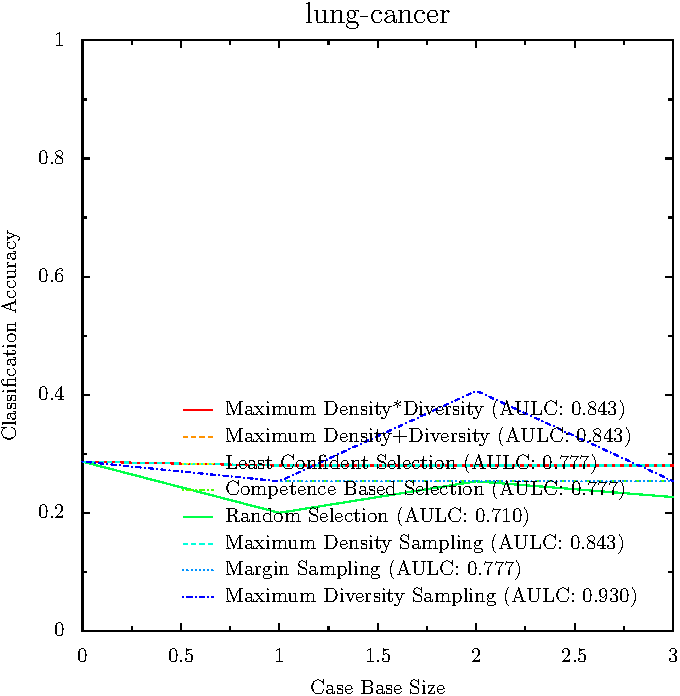
\includegraphics{./Plots/lung-cancer}
\caption{Learning Curve Plots for `Lung Cancer' Dataset (\ref{sec:lung_cancer})}
\end{figure}

\begin{figure}[h!]
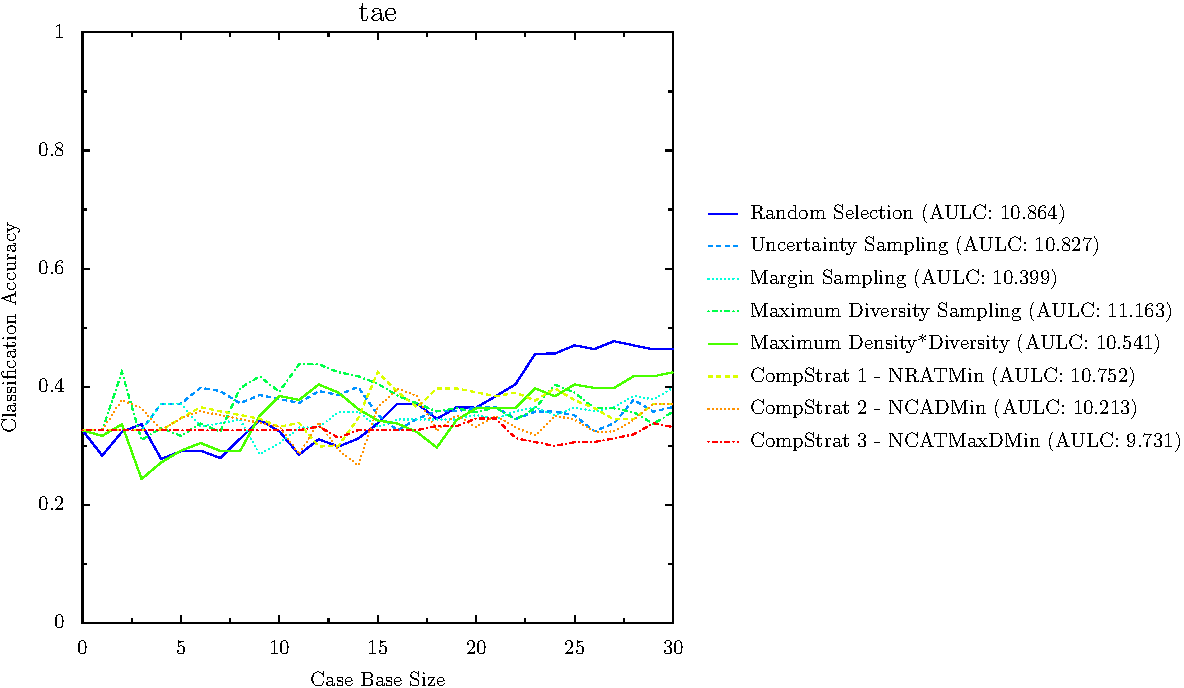
\includegraphics{./Plots/tae}
\caption{Learning Curve Plots for `TA Evaluation' Dataset (\ref{sec:taevaluation})}
\end{figure}

\begin{figure}[h!]
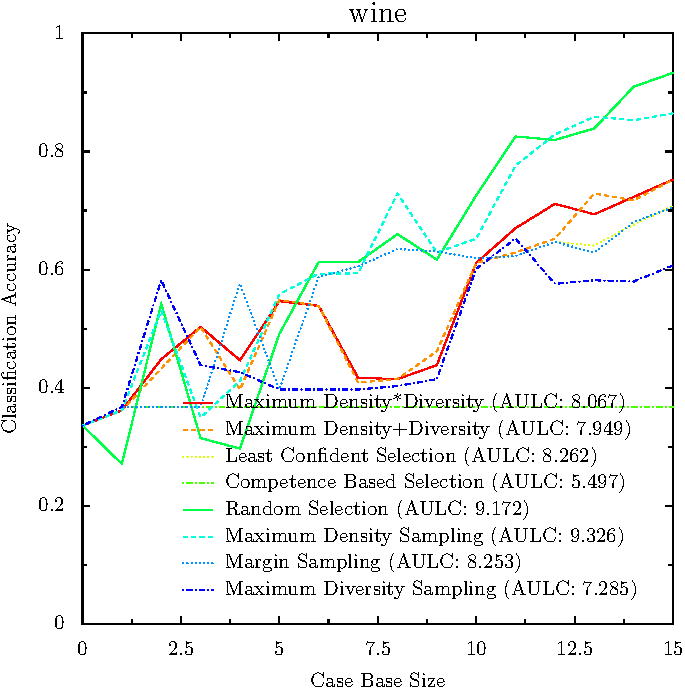
\includegraphics{./Plots/wine}
\caption{Learning Curve Plots for `Wine' Dataset (\ref{sec:wine})}
\end{figure}

\begin{figure}[h!]
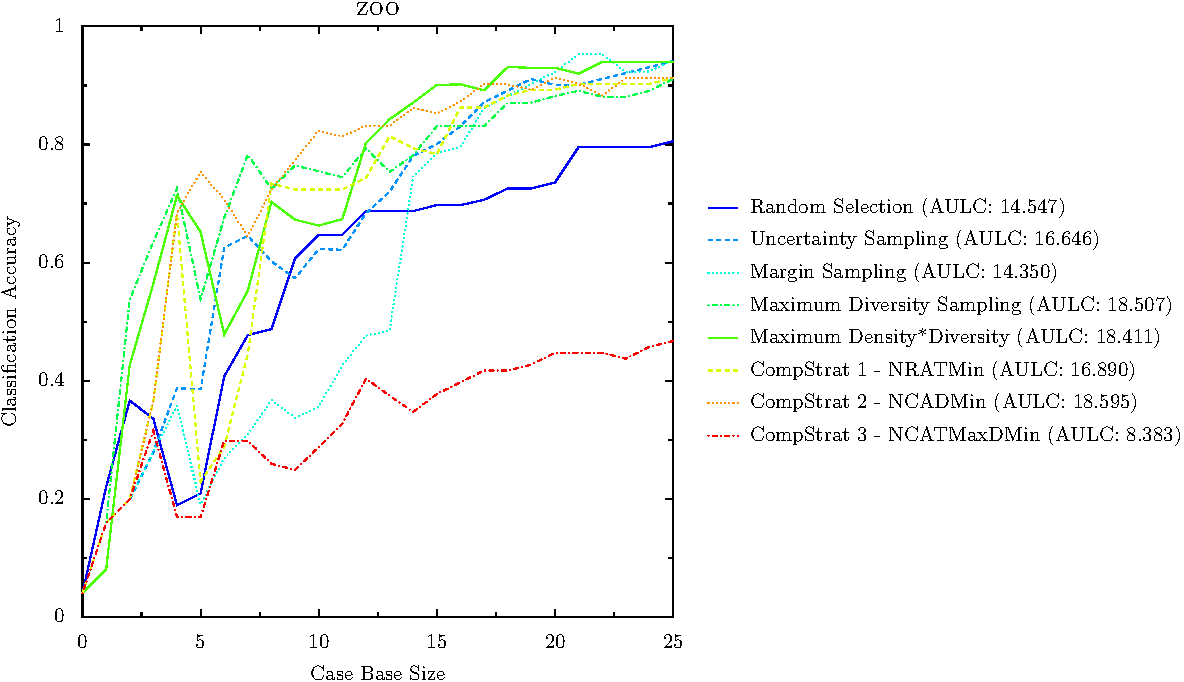
\includegraphics{./Plots/zoo}
\caption{Learning Curve Plots for `Zoo' Dataset (\ref{sec:zoo})}
\end{figure}

\subsection{Textual Datasets}

\chapter{Conclusions and Future Work\label{cha:conclusions}}

\section{Closing Opinions}
\subsection{Backing Source Code should always accompany Experimental Results}

\section{Possible Future Work Areas} \footnote{I'm staying away from simply saying ``Future Work'', since I have little to no intention of actually doing any of the following, unless it's actually something I want to progress in any future projects.}



(Start a revolution in the research community - code should always accompany the paper)

\chapter{Appendix}
\section{Open source Technologies Used}
%TODO Put in short description of each.
\subsection*{python}
\subsection*{git}
\subsection*{pypy}
\subsection*{orange}
\subsection*{pyx}
\subsection*{matplotlib}
\subsection*{Eclipse}
\subsection*{Pydev}
\subsection*{Aptana}
\subsection*{Dia}
\subsection*{Latex}
\subsection*{TexStudio}
\subsection*{Ubuntu}
\subsection*{SciKit Learn}
\subsection*{cProfile}
\subsection*{Run Snake Run}
\subsection*{bpython}
\subsection*{Lyx}
\subsection*{Graphviz}
\subsection*{PyGraphviz}
\subsection*{PyPdf}
\subsection*{Google Protocol Buffers}
\subsection*{PdfRider}
http://pdfrider.codeplex.com
Extracting pages
\subsection*{Briss}
http://sourceforge.net/projects/briss/ - pdf cropping
\subsection*{csvtools}
Deprecated (but useful!) latex package to import CSVs.

\subsection*{extraplaceins}
http://lexfridman.com/blogs/research/2011/03/06/prevent-figures-from-floating-outside-sections-in-latex/

\section{Cut Sections}
\subsection{Criticism against Reachability/Dissimilarity Sets}
A case either has a Reachability set, or Dissimilarity set - never both. This either-or nature is convenient for Delany's binary-style analysis, but throws away all information about the \emph{competing} set (be it Reachability, or Dissimilarity).

e.g. for Classes {y, n}, if:
\begin{itemize}
	\item $class(case_{1})=y$ 
	\item $k = 3$
	\item $class(NN_{1}(case_{1})) = y$ 
	\item $class(NN_{2}(case_{1})) = y$
	\item $class(NN_{3}(case_{1})) = x$  
\end{itemize}
and non-weighted voting is used, then it is correctly classified `y' and:
\begin{itemize}
	\item $reachability(case_{1})=\left\{ NN_{1}(case_{1}),\hphantom{}NN_{2}(case_{1})\right\} $
	\item $dissimilarity(case_{1})=\left\{ \right\} $
\end{itemize}

Here, no knowledge of $NN_{3}(case_{1})$ is maintained. I believe it would be more natural to have the Dissimilarity Set to include cases that were \emph{fighting} against the correct classification, even if the case was correctly classified.

\subsection{Smyth \& McKenna's Work on Competence Models}
\subsubsection{Introduction}
Barry Smyth and Elizabeth McKenna performed interesting research on using a clustering techniques to expand on the work of \citet{Smyth1995} \cite{Smyth1998}.

\subsubsection{Coverage}
Coverage is defined in terms of the Retrieval and Adaptation Spaces.

\paragraph{Retrieval Space}

These are simply the cases retrieved from the case base for a given case.

\[ RetrievalSpace(c \in C) = \left\{ c' in C : c' \text{ is retrieved for c} \right\} \]

\paragraph{Adaptation Space}

\[ AdaptationSpace(c \in C) = \left\{ c' \in C : c' \text{ can be adapted to solve } c \right\} \]

\paragraph{Coverage}

The Coverage of a case is defined as the intersection between that case's Retrieval and Adaptation Spaces. \footnote{Intersection because all of those that could be adapted to solve this case may not be retrieved, and ones may be retrieved that cannot be adapted (depending on the retrieval mechanism used).}

\[ Coverage(c \in C) = \left\{ c' \in C : c' \in RetrievalSpace(c) \cap AdaptationSpace(c) \right\} \]


\subsubsection{Competence Group}
The most interesting part of the paper is their notion of a Competence Group. They argue that the fundamental unit of competence should not be at the case level, but instead should be at a cluster level, where clustering is performed by the notion of Shared Coverage.

Two cases exhibit Shared Coverage if their Coverage Sets overlap. A Competence Group is then defined as a maximal  collection  of  cases  exhibiting  shared Coverage \footnote{Of particular note here is that maximal means that it is not necessary that each set intersect directly with every other set - but that each case in the group is simply \emph{reachable} by means of Shared Coverage links by every other case in the group. In graph terms, we would speak of the graph's components - each component a maximally connected set of nodes - with an edge between two nodes representing Shared Coverage between those two nodes.}.

\subsubsection{Case \& Group Density}

Case Density as per Smyth and McKenna's definition is a case's Average Similarity with the other things in a given group. \footnote{Similarity is taken to be a function that, given 2 cases, computes the similarity between those two cases on a scale from 0 to 1, where 0 is in no way similar, and 1 is exactly the same.}

\[
CaseDensity(c,G)=\frac{\underset{c'\in G-\{c\}}{\sum}Sim(c,c')}{\left|G\right|-1}
\]

Group density they define as the average similarity of each thing in the group with the rest of the group from 0 to 1 - i.e. on average how similar are the things in the group to each another.

\[
GroupDensity(G)=\frac{\underset{c\in G}{\sum}CaseDensity(c,G)}{\left|G\right|}
\]

\subsubsection{Group Coverage}
The competence measure of a group of cases is that of Group Coverage, and is defined as follows:

\[
GroupCoverage(G)=1+\left[\left|G\right|\bullet(1-GroupDensity(G))\right]
\]

Intuitively - it's bad to have a lot of redundancy, so we want things to be not too close together - therefore \emph{goodness} is inversely proportional to average similarity. Larger groups (as long as not dense) give greater coverage - therefore directly proportional to size.

Actual Reasoning could be looked on as follows:
\begin{itemize}
	\item GroupDensity gives average similarity within the group (from 0 to 1 - 0 being not at all similar, 1 being exactly the same).
	\item 1-Group Similarity gives average dissimilarity within the group.
	\item Multiplying this average by G the total dissimilarity between the members of the group. \footnote{Another way of looking at it - gives a \emph{strength} of how relevant this group is. (e.g. a group of 2 needs to be taken with a pinch of salt vs a group of 1,000)}
	\item 1 added for when no dissimilarity (either identical cases or single case in the group), these should still have weighting.
\end{itemize}

\subsubsection{Case Base Coverage}
The overall case base coverage (on which case base competence is believed in the paper to follow) as simply the sum of the Group Coverages of all the individual Competence Groups in the case base.

\[
Coverage(G)=\underset{G_{i}\in G}{\sum}GroupCoverage(G_{j})
\]

\subsubsection{Experimental Conclusions}
Smyth and McKenna found a close correspondence between their Case Base Coverage competence model, and the true competence of the case base against the test sets\cite{Smyth1998}.

\subsubsection{Comments}
Smyth and McKenna's general argument on how it is difficult to establish an individual case's competence seems valid. It is much more natural to define competence characteristics based on groups of cases. 

Traditionally, when talking about grouping, it seems to have been done through clustering, or simply at the case level by having the notion of a case's neighbourhood (which can be defined in various ways - such as within a radius, the k nearest, etc.).

The notion of defining competence groups through graph-style application of maximally connected components is an interesting one. Here, specifically, edges are based on Shared Coverage, but one can easily see how this approach could be applied based on other criteria to represent an edge.

\bibliographystyle{plainnat}
\bibliography{library}
\end{document}